\chapter{Mask Training}
\label{chap:chapter2}


\localtableofcontents


\begin{abstract}

  This chapter focuses on the development of lightweight and efficient neural
  networks for image classification tasks, particularly in visual category
  recognition. These lightweight networks are increasingly important for
  intelligent embedded systems with limited computational and energy resources.
  Pruning techniques are popular in designing lightweight networks, but they
  require weight training, pruning and fine-tuning. These weights are pruned
  based on criteria or saliency indicators that are learned alongside the
  weights.
  
  This chapter introduces approaches that extract effective subnetworks by
  pruning large untrained networks, without weight training. A new method, named
  \acf{ASLP}, is proposed to extract effective subnetworks from a large,
  untrained deep neural network using the \acf{STGS} technique, which enables
  stochastic computation graphs to be trained with discrete variables while
  still preserving differentiability. Additionally,a weight rescaling mechanism,
  referered to as \acf{SR}, is introduced. It rescales the weight distributions
  of the selected subnetworks and as a result, improves the performance and
  reduces the number of epochs required for training as shown later in
  experiments. Finally, we introduce a novel pruning strategy that automatically
  finds the pruning rate yielding the best performances once the training
  complete, eliminating the need to iteratively search and strictly enforce of a
  specific pruning rate throughout the training.\\

  The \ac{ASLP} method, which integrates the \ac{STGS} sampling technique and
  the \ac{SR} mechanism, is evaluated through experiments on CIFAR-10,
  CIFAR-100, and TinyImageNet datasets. In most cases, \ac{ASLP} outperforms
  other state-of-the-art methods and consistently surpasses them for various
  network architectures. Further experiments show that the sparsity of the
  networks extracted with \ac{ASLP} can be increased with minimal impact on the
  performance. These experiments also show that our method can accept a broad
  range of learning rates and is robust to extremely large learning rate values.
  Additionally, the experiments show the effectiveness of the \ac{SR} mechanism
  regarding the performance improvement and the reduction in the number of
  epochs needed to reach convergence.\\

  \noindent This chapter presents work that has resulted in the publication of the
  following conference article:
  \bibentry{DBLP:conf/icip/DupontASL22}
  \begin{itemize}
    \item Robin Dupont, Mohammed Amine Alaoui, Hichem Sahbi, and Alice
          Lebois. Extracting effective subnetworks with Gumbel-Softmax. In \textit{2022
            IEEE International Conference on Image Processing, ICIP 2022, Bordeaux,
            France, 16-19 October 2022,} pages 931–935. IEEE, 2022.
  \end{itemize}

  \noindent Our code for the \ac{ASLP} method, as well as the reimplementation
  of the comparative methods used in this chapter, is publicly available at:
  \begin{itemize}
    \item \url{https://github.com/N0ciple/ASLP}
  \end{itemize}

\end{abstract}

\section{Introduction and Related Work}
% region: introduction

In this chapter, we tackle the challenge of extracting lightweight and effective
subnetworks from large, untrained neural networks. The goal is to obtain
subnetworks that have both a smaller number of parameters compared to the
original network and compelling performances. Contrary to \cref{chap:chapter1}
where the focus was on soft-pruning weights based on their value during the
training, the method presented in this chapter relies on training latent masks.
The latter represents a parametrisation of the probabilities for the weights to
be selected or not in a sampled topology. The method described in
\cref{chap:chapter1} binds the saliency of the weights to their magnitude in a
fully deterministic way. In contrast, the method introduced in this chapter is,
on the one hand, stochastic, and on the other hand, decorrelating the pruning
criterion from the weight value by relying on a separate latent mask to
represents the weight saliency.\\

This method exhibits several advantages over the method presented in the
previous chapter: First, as we just mentioned, the pruning criterion is
decorrelated from the value of the weight, offering a different approach where
the weight value is not the only parameter determining its saliency. Indeed, two
weights with the same value can have different probabilities of being selected
since their associated latent mask can evolve differently. Second, this method
does not train the weights but selects the best subset of network connections to
minimise the loss used to train the network. Consequently, this method is
perfectly suited for applications where training the weight might not be
possible and activating or deactivating a weight is the only option. Finally,
from a global standpoint, this method provides a new path to neural network
training that does not rely on weight training, but rather on topology selection
through the same widely spread gradient-based optimisation framework used by
standard training.\\

%TODO: compléter l'intérêt de ce nouveau "chemin" ?

% \subsection{Related Work}\label{sec:chap2:related_work}


\subsection{Pruning at initialisation} 

In general, extracting an efficient subnetwork is still an challenging problem
\cite{frankle2020pruning} and is computationally demanding as this amounts to
full training of large networks (until convergence) prior to their pruning.
Instead of pruning the network after an initial training phrase, existing
alternatives approach this problem by pruning the network weights just after
their initialisation and before training
\cite{DBLP:conf/iclr/LeeAT19,DBLP:conf/iclr/WangZG20,DBLP:conf/nips/TanakaKYG20}.
The resulting sparse network is then trained after this initial pruning step, as
shown in \cref{fig:chap2:pipelines_pruning_at_initialisation}.\\

\begin{figure}[htbp]
  \centering
  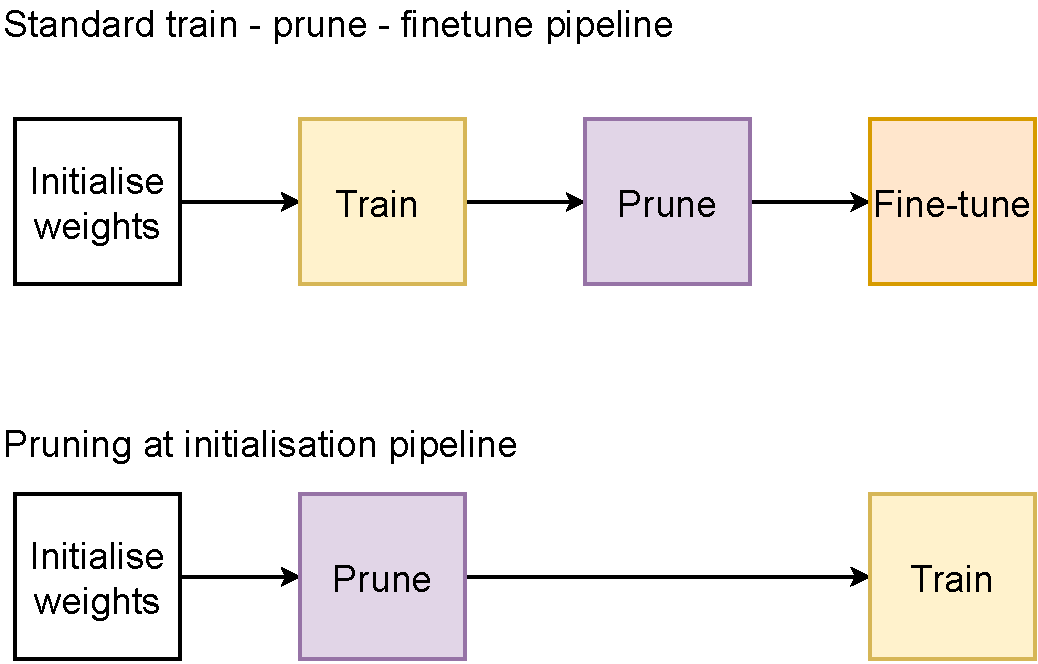
\includegraphics[width=0.7\textwidth]{chapter_2/assets/prune_at_init_pipeline.pdf}
  \caption{Comparison of a standard \emph{train-prune-finetune} pipeline and the
  \emph{prune at initialisation} pipeline. In the latter, the network is pruned
  before training.}
  \label{fig:chap2:pipelines_pruning_at_initialisation}
\end{figure}

Single-Shot Network Pruning (SNIP) was introduced by
\citeauthor{DBLP:conf/iclr/LeeAT19} in \cite{DBLP:conf/iclr/LeeAT19}. The
authors devise a new criterion to determine the importance of a connection even
before the start of training. The criterion, called \emph{connection
sensitivity}, is based on the influence of a connection on the loss function.
The more a connection can change the loss function output, the more important it
is considered to be. Considering a weight $w_j$, the authors define its
sensitivity as:\\

\begin{equation}
  \label{eq:snip}
  % Old style
  % s_j=\displaystyle\frac{|g_j(\bf{w};\mathcal{D})|}{\displaystyle\sum_{k=1}^m |g_{k}(\bf{w};\mathcal{D})|}
  % New style
  s_j = \displaystyle\frac{\left|\displaystyle\frac{\partial \mathcal{L}}{\partial c_j}\right|}{\displaystyle\sum_{k=1}^N \left|\displaystyle\frac{\partial \mathcal{L}}{\partial c_k}\right|}
\end{equation}\\

\noindent where $N$ is the number of connections in the network and $c_j$ in an
auxiliary variable introduced by the authors that represents the presence
($c_j=1$) or absence ($c_j=0$) of the weight $w_j$ in the network. The
connections are then sorted by their connection sensitivity score and the
top-$k$ connections are kept to match a given pruning rate.\\

GraSP (Gradient Signal Preservation) \cite{DBLP:conf/iclr/WangZG20} is a
refinement of SNIP that takes into account the \emph{gradient flow}. The authors
seek to preserve the latter in order to allow large gradients in the subsequent
network training. The scores of the weights are defined in a vectorised way as
:\\

\begin{equation}
  \label{eqn:chap2:grasp_score}
  \bf{S}(-\bf{w}) = -\bf{w} \odot \bf{H} \bf{g}
\end{equation}\\

\noindent where $\odot$ is the Hadamard product, $\bf{w}$ is the vector of
weights, $\bf{H}$ is the Hessian matrix of the loss function with respect to the
weights and $\bf{g}$ is the gradient of the loss function with respect to the
weights. Considering how the score is defined in \cref{eqn:chap2:grasp_score},
pruning is achieved by removing the top-$k$ weights that reduce the gradient
flow to match a given pruning rate.\\

Both SNIP and GraSP require a single mini-batch to compute their respective
scrores. Another pruning method known as SynFlow
\cite{DBLP:conf/nips/TanakaKYG20} is data-free and seeks to preserve
\emph{synaptic flow}, defined subsequently, in a given  network in order to
prevent \emph{layer-collapse}. The latter is defined by the authors as the
complete pruning of a layer, which effectively renders the network untrainable.
For a given layer $\ell$, the \emph{synaptic flow} score of the weights
$\theta_\ell$ of a layer $\ell$ is defined as :\\

\begin{equation}
  \label{eqn:chap2:synflow_score}
  % old style
  % \mathcal{S}_\text{SF}(\theta_\ell) = \displaystyle\frac{\partial ~ \left(\mathbb{1}^T \left( \displaystyle\prod_{\ell=1}^{L} | \theta_\ell | \right) \mathbb{1}\right)}{\partial ~ \theta_\ell} \odot \theta_\ell
  % new style
  \mathcal{S}_\text{SF}(\mathbf{w}_\ell) = \displaystyle\frac{\partial ~ \left(\mathbb{1}^T \left( \displaystyle\prod_{\ell=1}^{L} | \mathbf{w}_\ell | \right) \mathbb{1}\right)}{\partial ~ \mathbf{w}_\ell} \odot \mathbf{w}_\ell
\end{equation}\\

\noindent where $L$ is the total number of layers in the network and
$\mathbb{1}$ is the all ones vector. In contrary to previous methods, namely
SNIP \cite{DBLP:conf/iclr/LeeAT19} and GraSP \cite{DBLP:conf/iclr/WangZG20},
SynFlow does not necessitate any data to compute the scores. These scores are
computed and updated iteratively for 100 iterations, regardless of the targeted
dataset or batch size. Since it prevents layer-collapse, networks pruning with
SynFlow can reach higher pruning rates than with SNIP or GraSP (see
\cref{fig:chap2:synflow_perfs}).\\

\begin{figure}[htbp]
  \centering
  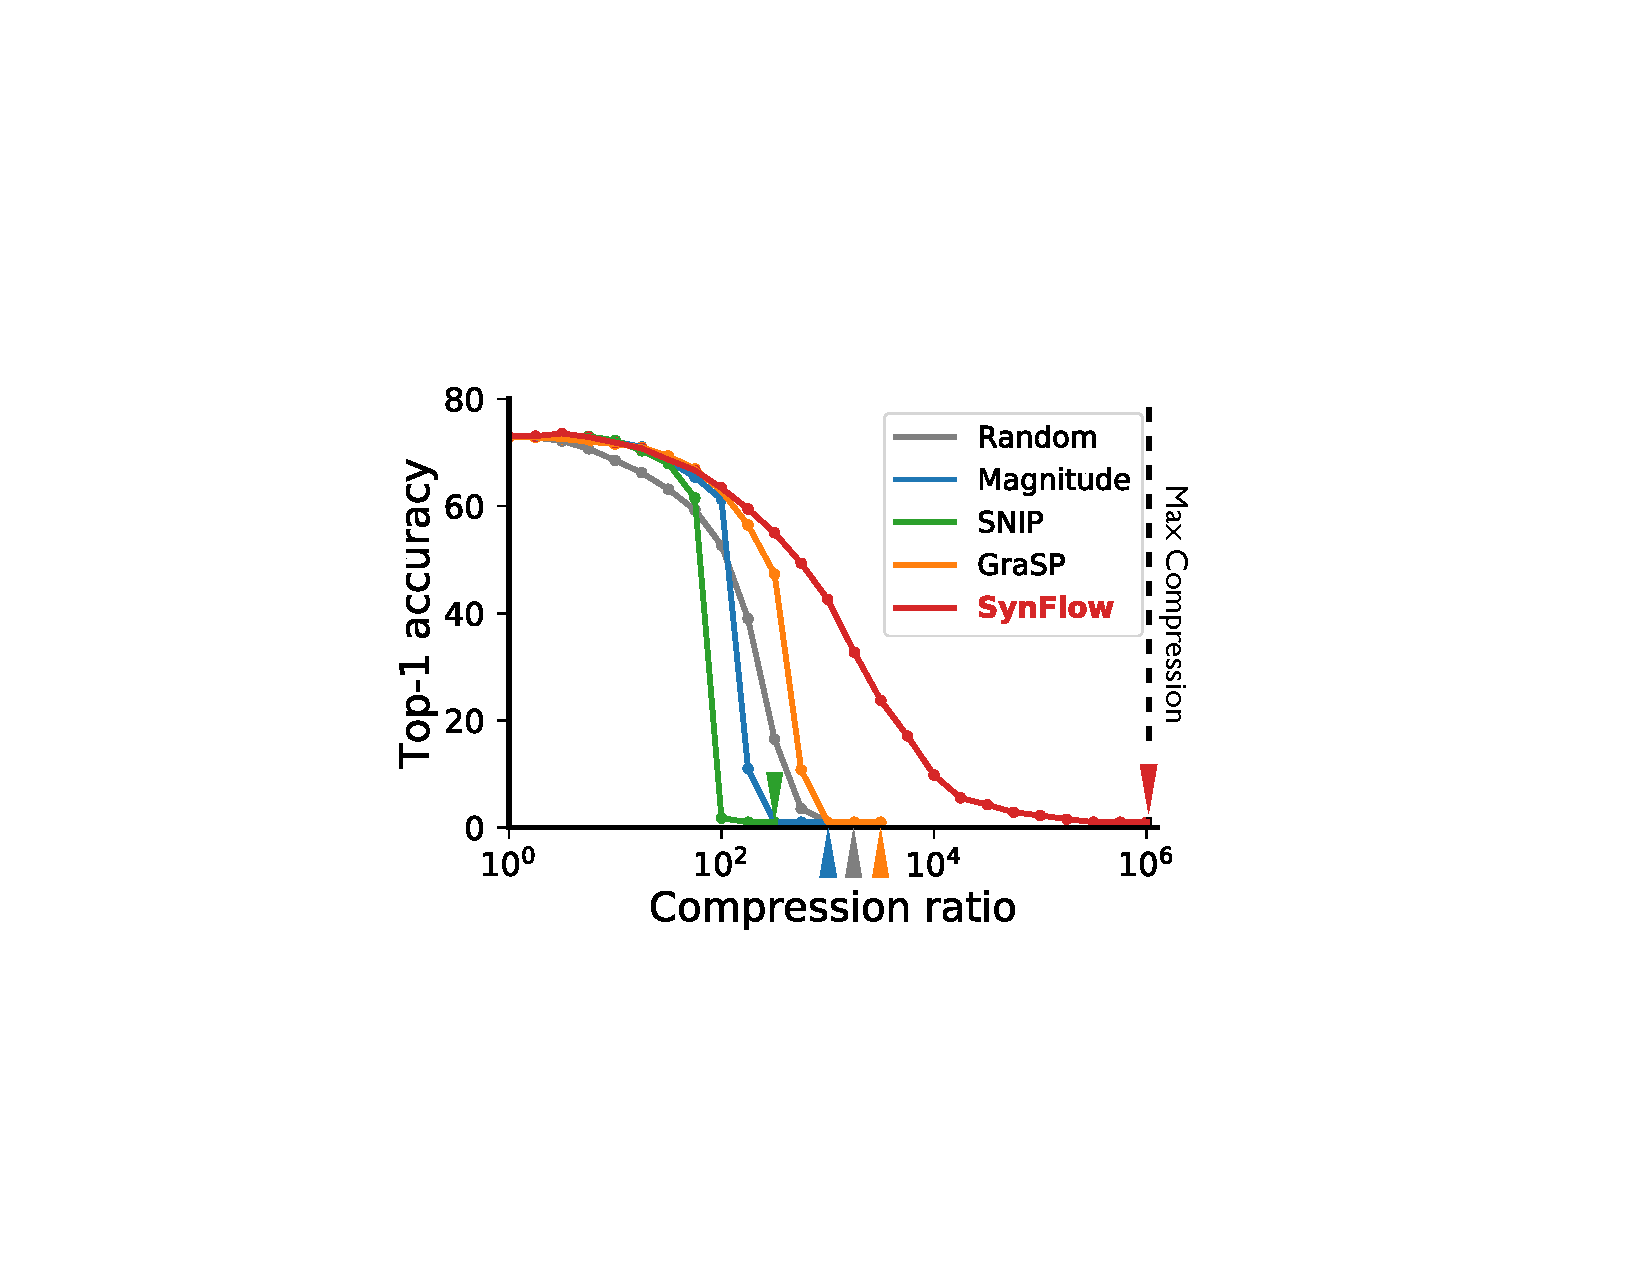
\includegraphics[width=0.7\textwidth]{chapter_2/assets/synflow_perfs.pdf}
  \caption{Synflow accuracy compared to SNIP and GraSP for different pruning
  rates. Methods are benchmarked on VGG16 trained on CIFAR-100. Illustration
  taken from \cite{DBLP:conf/nips/TanakaKYG20}} 
  \label{fig:chap2:synflow_perfs}
\end{figure}

These aforementioned methods allow to prune a network at initialisation, but
still require training the weights. Moreover, while these methods outperform the
basic benchmark of random pruning, their accuracy is still below the one of
post-training magnitude pruning \cite{frankle2020pruning}. In contrast to these
works, our proposed solution in this chapter identifies effective subnetworks by
training only their topology and without any weight tuning. Our solution yields
sparse and lightweight subnetworks that achieve compelling performances and does
not need further weight fine-tuning.\\

\subsection{Lottery Tickets} 
As discussed in \cref{chap:chapter1,chap:sota}, pruning methods, either
structured or unstructured, are particularly successful at simplifying large
neural networks, and seek to remove connections with the least perceptible
impact on classification accuracy. Structured pruning consists in {\it jointly}
removing groups of weights, entire channels or subnetworks
\cite{DBLP:conf/iclr/0022KDSG17, DBLP:conf/iccv/LiuLSHYZ17}, whereas
unstructured pruning aims at removing weights {\it individually}
\cite{DBLP:conf/nips/HanPTD15,DBLP:journals/corr/HanMD15}.\\

Unstructured pruning has witnessed a recent surge in interest in the wake of the
\ac{LTH} \cite{DBLP:conf/iclr/FrankleC19}; an empirical study in
\cite{DBLP:conf/iclr/FrankleC19} demonstrates that large pre-trained networks
encompass lightweight subnetworks, referred to as \textit{\acp{LT}}, which can
achieve comparable performance to the original large networks in a similar
number of epochs when trained in isolation with initial weights taken from the
large network. To identify these \acp{LT}, the large network is trained until
convergence, followed by pruning the smallest weights based on their magnitude.
The remaining weights are then rewound to their original value, that is, the
value they had before the training of the large network began. This resulting
subnetwork is known as a \textit{Lottery Ticket}.
\citeauthor{DBLP:conf/iclr/FrankleC19} also leveraged \emph{iterative magnitude
pruning} to identify \acp{LT}, where the pruning rate is gradually increased
during training until it reaches the desired pruning rate
\cite{DBLP:conf/iclr/FrankleC19}.\\

Rewinding the weights to their original values does not allow to find \ac{LT}
for larger architectures, as noted by
\cite{DBLP:conf/iclr/LiuSZHD19,DBLP:journals/corr/abs-1902-09574}.
\citeauthor{DBLP:conf/iclr/FrankleC19} proposed a weaker version of the \ac{LTH}
where the weight values are not reset to their original values, but instead to
an early stage of the training corresponding to the network reaching a stable
state, described in \cite{DBLP:conf/icml/FrankleD0C20}.
\Cref{fig:chap2:lt_schemes} provides conceptual illustrations of the different
existing methods devised by \citeauthor{DBLP:conf/iclr/FrankleC19} to find a
\ac{LT}.\\

\begin{figure}[htbp]
  \centering
  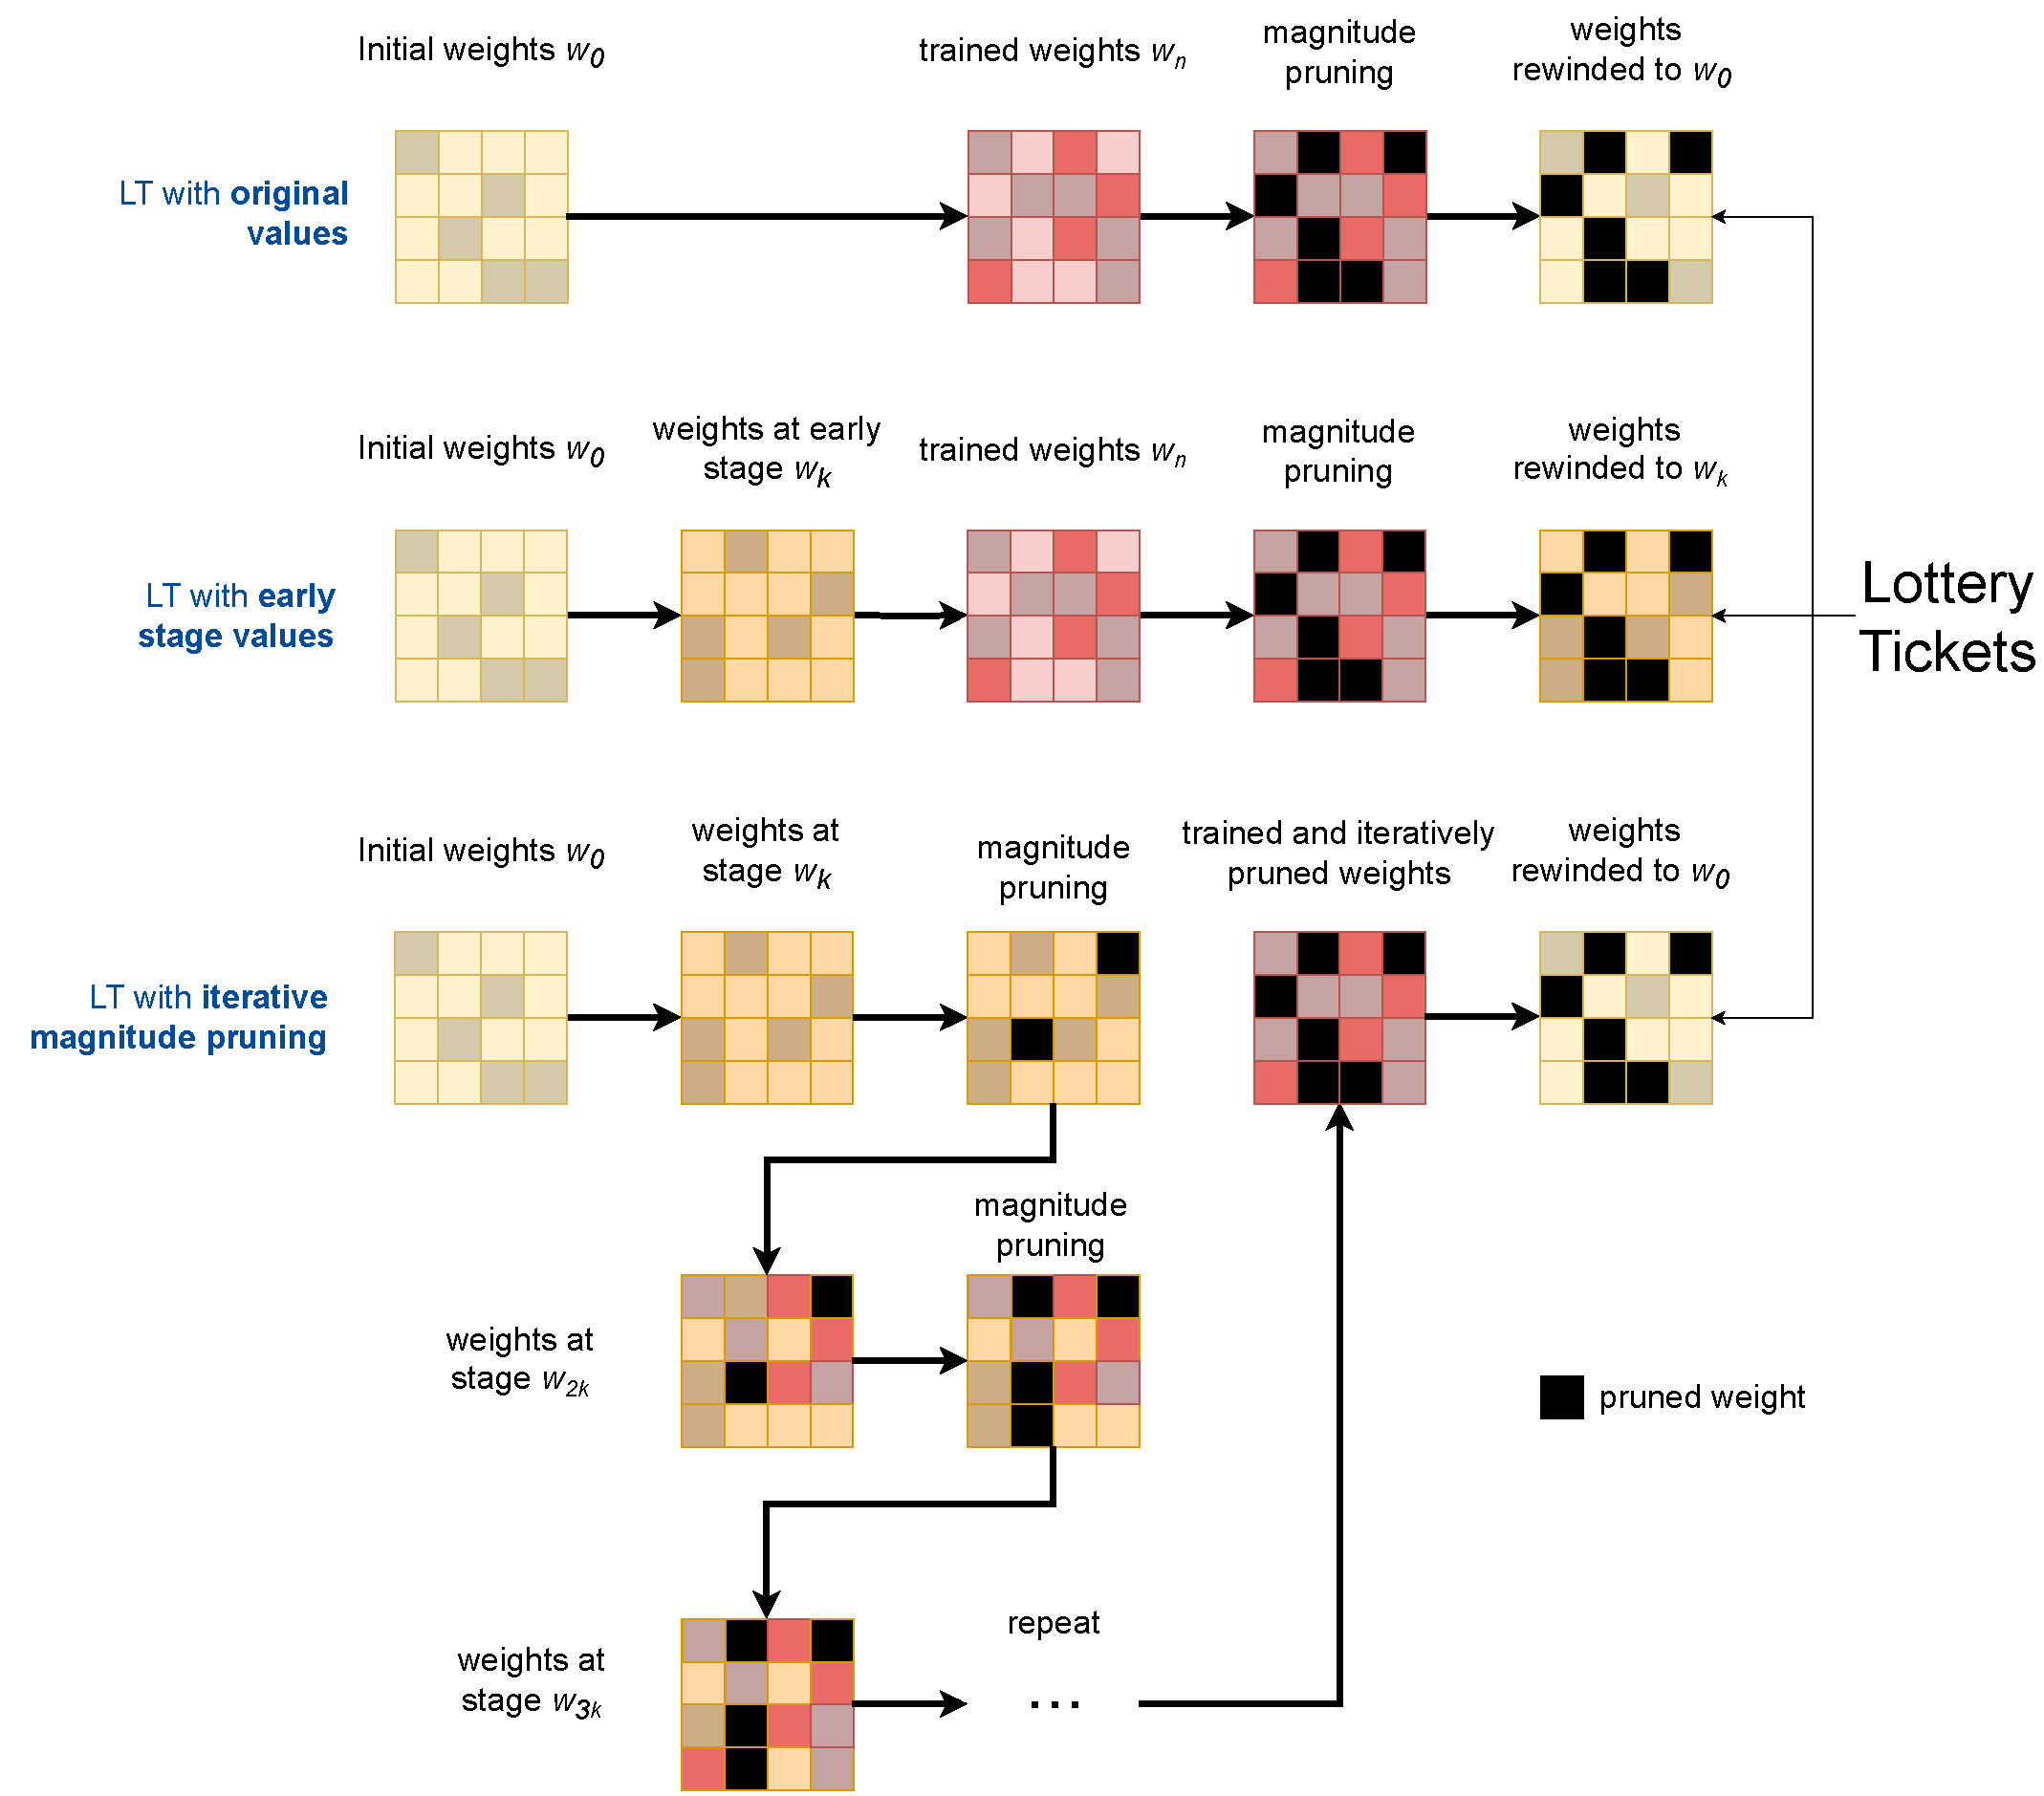
\includegraphics[width=\textwidth]{chapter_2/assets/LT_schemes.pdf}
  \caption{Conceptual illustration of the different processes to obtain a
  \acl{LT}: reinitialising the weights to their original values with one-shot
  magnitude pruning (\emph{LT with original values}), reinitialising the weights
  to their early stage values with one-shot magnitude pruning (\emph{LT with
  early stage values}) and iterative magnitude pruning (\emph{LT with iterative
  magnitude pruning}). Best viewed in colour.}
  \label{fig:chap2:lt_schemes}
\end{figure}

Another study \cite{DBLP:conf/iclr/LiuSZHD19} pushes that finding further and
concludes that only the topology of these subnetworks is actually important in
order to reach compelling performances. \citeauthor{DBLP:conf/iclr/LiuSZHD19}
\cite{DBLP:conf/iclr/LiuSZHD19} point out that the weights of the \acp{LT} are
not important and can be randomly initialised, provided that the optimisation
procedure is carefully designed: \citeauthor{DBLP:conf/iclr/LiuSZHD19} used a
common \ac{SGD} optimiser with momentum instead of using an Adam optimiser
\cite{kingma2014adam} with low learning rate as
\citeauthor{DBLP:conf/iclr/FrankleC19} did in \cite{DBLP:conf/iclr/FrankleC19},
suggesting that using an Adam optimiser might hinder the training of randomly
initialised \ac{LT}.\\

The aforementioned works
\cite{DBLP:conf/iclr/FrankleC19,DBLP:conf/icml/FrankleD0C20,DBLP:conf/iclr/LiuSZHD19}
focus on finding a \acl{LT} that still needs to be trained in order to reach a
satisfying level of performance. In contrast, our proposed method extracts a
subnetworks that already achieves compelling performances without any weight
training.\\ 


\subsection{Existence of effective subnetworks} 
At first, it seems counterintuitive that there exists a subnetwork in a large
network, that can achieve compelling performances without any weight training.
This has been first conjectured in \cite{DBLP:conf/cvpr/RamanujanWKFR20} as the
Strong \acl{LTH}. A few theoretical analyses provide evidence that such
subnetworks do exist. \cite{DBLP:conf/icml/MalachYSS20} demonstrate that a
neural network of width $d$ and depth $l$ can be approximated by pruning a
randomly initialised one that is a factor $O(d^4l^2)$ wider and twice as deep.
The  upper bound on the network width has later been improved by
\cite{DBLP:conf/nips/OrseauHR20} to $O(d^2\log(dl))$ under the assumption of a
hyperbolic weight distribution. This upper bound has eventually been refined to
$O(d\log(dl))$ by \cite{DBLP:conf/nips/PensiaRNVP20} for a broad class of weight
distributions, including the uniform one which is widely used for weight
initialisation \cite{DBLP:conf/iccv/HeZRS15}.\\

\subsection{Subnetwork topology extraction}\label{sec:chap2:subnetwork_topology_extraction}
Although the existence of effective subnetworks with untrained weights has been
established, no constructive proof has been provided in order to identify them.
In this context, several methods proposed heuristics to extract the lightweight
and efficient subnetwork from a large untrained network
\cite{DBLP:conf/nips/ZhouLLY19,DBLP:conf/cvpr/RamanujanWKFR20}.\\

Supermark is a method introduced by \citeauthor{DBLP:conf/nips/ZhouLLY19} in
\cite{DBLP:conf/nips/ZhouLLY19} which is the first attempt to extract efficient
subnetworks from a large untrained network using stochastic mask training. The
weights of the network are stochastically sampled following a Bernoulli
distribution parametrised by a latent variable $m$. To that extent, weights are
reparametrised as follows:
\begin{equation}
  \label{eqn:chap2:sigmoid_reparam}
  \hat{w} = w_i \odot \text{Bern}(\sigma(m))
\end{equation}
where $\hat{w}$ is the \emph{effective weight} (also referred to as the
\emph{apparent weight} in \cref{chap:chapter1}) used in the network, $w_i$ is
the original frozen weight, $\odot$ denotes the element-wise product and
$\sigma$ the sigmoid function. At each iteration, a random variable is sampled
from the Bernoulli distribution parametrised by $m$, that either selects or
prunes the corresponding weight. The sampling being nondifferentiable, it is not
possible to train directly $m$ with \ac{SGD}. Instead, the authors proposed to
use the \ac{STE} \cite{DBLP:journals/corr/BengioLC13}, a technique that
approximates the gradient in the backward pass with a continuous surrogate
function of the forward pass non-differentiable function.
\citeauthor{DBLP:conf/nips/ZhouLLY19} also introduced a weight rescaling
mechanism, called \ac{DWR}, to mitigate the disruption of weight statistics due
to pruning \cite{DBLP:conf/iccv/HeZRS15}. More details are given in
\cref{sec:chap2:stochastic-sampling,sec:chap2:smart-rescale}.\\


During training, weights are frozen and only the masks are allowed to vary.
However, the major drawback of this method resides in the vanishing gradient
issue of the sigmoid which makes mask training numerically challenging.
\citeauthor{DBLP:conf/cvpr/RamanujanWKFR20}
\cite{DBLP:conf/cvpr/RamanujanWKFR20} proposed another alternative, entitled
Edge-popup, based on binarised saliency indicators learned with \ac{STE}, which
selects the most prominent weights in the resulting subnetworks. Each weight
$w_{ij}$ is associated with a latent saliency indicator $s_{ij}.$ During the
forward pass, the weights associated with the top-$k$ saliency indicators are
selected and the others are pruned. Similarly to Supermask, binarised saliency
indicatord are not differentiable, therefore, the latter is made with \ac{STE}.
The authors consider the following expression for the weights in the backward
pass:
\begin{equation}
  \hat{w}_{ij} = s_{ij} w_{ij}
\end{equation}
Edge-popup enforces the pruning rate \textit{a priori}, thereby determining the
value of $k$. This value is the same for all the layers, imposing a constant
pruning rate throughout all the layers of the network, which is suboptimal.
Indeed, the optimal pruning rate is layer-dependent and varies from one layer to
another. Moreover, finding the pruning rate giving the highest performances has
to be made through a cumbersome and time-consuming grid search. Like Supermask,
Edge-popup also includes a weight rescaling mechanism, based on a learnt
rescaling factor that rescale the weight distribution in a layer-wise fashion,
subsequently detailed in \cref{sec:chap2:smart-rescale}.\\

\section{Contributions}
\label{sec:chap2:intro_contributions}

Considering the limitation of the aforementioned related work, namely, the
challenges in mask training due to the sigmoid mask parametrisation, and the
time-consuming nature of finding the optimal pruning rate, we introduce in this
chapter a new stochastic subnetwork selection method based on \ac{GS}. The
latter allows sampling subnetworks whose weights are the most relevant for
classification. The proposed contribution also relies on a new mask
parametrisation, entitled \acf{ASLP}, that allows better conditioning of the
gradient and thereby mitigates numerical instability during mask optimisation.
Besides, when combining \ac{ASLP} with a learned weight rescaling mechanism,
training is accelerated and the accuracy of the resulting subnetworks improves
as shown later in experiments. Our proposed pruning strategy is designed such
that it does not necessitate any prior information regarding the optimal pruning
rate that would yield the best performance. Instead, it automatically sets the
optimal rate, eliminating the need for exhaustive grid search.\\ 

The rest of this chapter is organized as follows: \cref{sec:chap2:method} delves
into our proposed method, named \acf{ASLP}, for extracting efficient subnetworks
using \acl{GS}, including stochastic weight sampling and our weight rescaling
approach. The overall workflow of our proposed method is detailed in
\cref{sec:chap2:overview}. In \cref{sec:chap2:experiments}, we share the results
of our comprehensive experiments, including performance benchmarks, the impact
of our weight rescaling approach, the effect of increased a posteriori sparsity,
and the impact of the learning rate on the training convergence speed and final
performance. We conclude the chapter in \cref{sec:chap2:conclusion}, summarizing
our contributions and our key findings. As we will demonstrate, our new approach
overcomes several of the challenges associated with previous techniques,
offering a more efficient and effective way to extract high-performance
subnetworks without weight training.


\section{Extracting Effective Subnetworks with Gumbel-Softmax}\label{sec:chap2:method}
% region: method

Considering the same formalism as in \cref{chap:chapter1}, let $f_\theta$ be a
deep neural network whose weights are defined as $\theta =
  \left\{\bm{w}_1,\mathellipsis, \bm{w}_L \right\}$, with $L$ being its depth,
$\bm{w}_\ell \in \mathbb{R}^{d_{\ell} \times d_{\ell-1}}$ its $\ell^\textrm{th}$
layer weights, and $d_\ell$ the dimension of $\ell$. The output of a given layer
$\ell$ is defined as \\

\begin{equation}
  \label{eqn:chap2:layer_eq}
  \mathbf{z}_{\ell} = g_\ell(\bm{w}_\ell \otimes \mathbf{z}_{\ell-1}),
\end{equation}\\

being  $g_\ell$ an activation function and $\otimes$ the usual matrix product.
Without loss of generality, we omit the bias in the definition of
(\ref{eqn:chap2:layer_eq}).

% ------------------------------------------------------------------------------
\subsection{Stochastic Weight Sampling}
\label{sec:chap2:stochastic-sampling}
% region: stochastic-sampling
\indent Given a network $f_\theta$, weight pruning consists in removing
connections in the graph of $f_\theta$. A node in this graph refers to a neural
unit while an edge corresponds to a cross-layer connection. Pruning is usually
obtained by freezing and zeroing out  a subset of weights in $\theta$, and this
is achieved in practice by multiplying $\bm{w}_\ell$ by a binary mask
$\bm{m}_\ell \in \{ 0,1 \}^{\text{dim}(\bm{w}_\ell)}$. The binary entries of
$\bm{m}_\ell$ are set depending on whether the underlying layer connections are
kept or removed, so \cref{eqn:chap2:layer_eq} becomes\\

\begin{equation}
  \label{eqn:chap2:pruned_layer_eq}
  \mathbf{z}_{\ell} = g_\ell( (\bm{m}_\ell \odot \bm{w}_\ell ) \otimes \mathbf{z}_{\ell-1} ).
\end{equation}\\

Here $\odot$ stands for the element-wise matrix product. In
\cref{chap:chapter1}, the \emph{effective pruning} step was achieved by setting
the values of $\bm{m}_\ell$ to zero or one depending on the magnitude of the
weight reparametrisation (see \cref{eqn:chap1:reparam,sec:chap1:overview}).
Consequently, the masks $\bm{m}_\ell$ values are only determined by the weights
values and not the topology of the network. In this chapter, we propose another
approach to obtain the masks $\bm{m}_\ell$ that is not bound to the weights
values. In \cref{eqn:chap2:pruned_layer_eq}, the masks $\bm{m}_\ell$
are stochastic and sampled from a Bernoulli distribution. However, sampling is
not a differentiable operation, therefore, optimising directly
${\bm{m}_\ell}$ is not possible. To overcome this issue, while still
relying on \ac{SGD}, the \acf{STE} technique is applied together with a
reparametrisation of the mask.\\

\noindent\textbf{\acl{STE}.} Zhou et al. \cite{DBLP:conf/nips/ZhouLLY19}
consider a Bernoulli parametrisation of $\bm{m}_\ell$ in order to
sample masks in \cref{eqn:chap2:pruned_layer_eq}. Since sampling is not a
differentiable operation, they rely on the \ac{STE}. It is a technique developed
in \cite{DBLP:journals/corr/BengioLC13} that enables the training of neural
networks with discrete activations, such as binary or quantised activations. The
technique involves using a differentiable relaxation to the non-differentiable
activation function during backward pass, and using the non-differentiable
function in the forward pass. This allows for the use of \ac{SGD} to optimise
the network, which was previously not possible with discrete activations. It is
worth noting that \ac{STE} is an heuristic that does not provide the correct
gradient, but it is effective in practice \cite{DBLP:journals/corr/BengioLC13}.\\

In order to apply \ac{STE} to the problem of Bernoulli stochastic mask
sampling, the definition of $\bm{m}_\ell$ is based on another
  {\it latent} parametrisation $\bm{\hat{m}}_\ell$, detailed
subsequently, and obtained by applying a sigmoid function $\sigma(.)$ to
$\bm{\hat{m}}_\ell$. This allows optimizing $\bm{\hat{m}}_\ell$  using gradient
descent by considering the following surrogate of
\cref{eqn:chap2:pruned_layer_eq} in the backward pass of the backpropagation
algorithm:\\

\begin{equation}
  \label{eqn:chap2:pruned_layer_eq2}
  \mathbf{z}_{\ell} = g_\ell( ( \sigma(\bm{\hat{m}}_\ell) \odot \bm{w}_\ell ) \otimes \mathbf{z}_{\ell-1} ).
\end{equation} \\

\noindent As a result, although masks $\bm{m}_\ell$ are sampled and thus
disconnected from the computation graph (sampling being not differentiable),
their reparametrisation $\bm{\hat{m}}_\ell$ can be updated as if they were used
in the computation graph as shown in \cref{eqn:chap2:pruned_layer_eq}.\\


\noindent\textbf{Gumbel-Softmax.} In what follows, we consider an alternative to
\ac{STE} based on \acf{GS} \cite{DBLP:conf/iclr/JangGP17} that demonstrates
better performances for differentiable categorical sampling, which is the
process of randomly selecting a category from a given set of categories, where
each category has a specified probability of being chosen. Gumbel-Softmax is a
technique that can be used to approximate a discrete categorical distribution
with a continuous relaxation. Gumbel-Softmax works by using the Gumbel
distribution \cite{gumbel1935valeurs} to add noise to a categorical distribution
and then applying the Softmax function to obtain a continuous relaxation of the
discrete distribution. The proposed method, dubbed as \acf{STGS}, is based on a
variant of \acl{GS} combined with \acl{STE}. In the forward pass, the softmax of
\ac{GS} is replaced by an argmax operator. Since this operator is not
differentiable, the standard softmax is considered in the backward pass. The
argmax operator allows sampling from a categorical distribution, as the limit of
\ac{GS} (\emph{i.e.}, when its softmax temperature approaches zero). \\

\noindent \textbf{Gumbel-Softmax applied to weight sampling.} Let $z$ be a
categorical random variable, associated with $n$-class probability distribution
$\mathcal{P} = [\pi_1,\dots,\pi_n]$. In order to sample in a differentiable
manner, the Gumbel-Softmax estimator takes as an input a vector of
log-probabilities \\

\begin{equation}
  \label{eqn:chap2:gumbel-softmax-input}
  \log(\mathcal{P}) =[\log(\pi_1),\dots, \log(\pi_n)]
\end{equation}\\

then it disrupts the latter with a random additive noise sampled from the Gumbel
distribution, and finally takes its argmax, yielding a categorical
variable. More formally, following \cite{DBLP:conf/iclr/JangGP17}, the value $q$
of our categorical variable $z$ is obtained as \\

\begin{equation}
  \label{eqn:chap2:gumbel-softmax-argmax}
  q = \underset{k}{ \text{argmax}} \ [ \log(\pi_k)+g_k ],
\end{equation}\\

with $g_k$ being independent and identically distributed samples from  the
Gumbel distribution with zero mean and unit variance, denoted
$\mathcal{G}(0,1)$.\\

For mask sampling, only two possible outcomes are considered. Either the
corresponding weight is selected and its mask is set to 1, or it is pruned from
the sampled topology and its mask is set to 0. In what follows, and unless
stated otherwise, we omit $\ell$ from $\bm{w}_\ell$ and we write it for short as
$\bm{w}$. Let $\bm{w}_{ij}$ be the weight associated with the i-th and j-th
neurons respectively belonging to layers $\ell-1$ and $\ell$. Since there are
two possible outcomes for the masks, we define a two-class categorical
distribution $\mathcal{P}_{ij}$ on $\{0,1\}$ as\\

\begin{equation}
  \left\{ \begin{array}{c}
    \mathcal{P}_{ij}(z=1)=\pi_1^{ij} \\
    \mathcal{P}_{ij}(z=0)=\pi_2^{ij}
  \end{array} \right.
\end{equation}\\

with, again, $\pi_1^{ij}=p_{ij}$ and $p_{ij}$ being the probability to keep the
underlying connection. Since there are only two mutually exclusive outcomes,
$\pi_2^{ij}=1-p_{ij}$. In other words, keeping the weight $\bm{w}_{ij}$ (or not)
in the sampled topology is a Bernoulli trial with a probability $p_{ij}$.
Considering \cref{eqn:chap2:gumbel-softmax-argmax}, a binary mask  $\bm{m}_{ij}$
is defined as\\

\begin{equation}
  \label{eqn:chap2:mask_value}
  \bm{m}_{ij} = 1_{\{q_{ij}=1\}}
\end{equation}\\

$1_{\{\}}$ being the indicator function and following
\cref{eqn:chap2:gumbel-softmax-argmax}, $q_{ij}$ is\\

\begin{equation}
  \label{eqn:chap2:q_ij_expression}
  q_{ij} = {\text{argmax}_{k \in \{1,2\}}}\big[\log(\pi_k^{ij})+g_k^{ij}\big]
\end{equation}\\

with $\pi^{ij}_1 = p_{ij}$ and $\pi^{ij}_2 = 1-p_{ij}$, the probability for a
weight to be selected or not in the sampled topology, respectively.\\

The proposed \ac{STGS} algorithm enables the learning of probabilities
$p_{ij}$ for each weight $\bm{w}_{ij}$ through \ac{SGD}. However, optimizing
$p_{ij}$ (with \ac{SGD}) raises a major issue. Since the optimisation is not
constrained, $p_{ij}$ can take values larger than 1 or smaller than 0. As a
consequence, it could no longer be interpreted as a probability, moreover,
$\log(p_{ij})$ and $\log(1-p_{ij})$ would also be undefined.\\

On another hand, solving constrained SGD, besides being computationally
expensive and challenging, may result in a worse local minimum. In order to
overcome all these issues, one may consider an alternative reparametrisation
$p_{ij}=\sigma(\bm{\hat{m}}_{ij})$, similar to the reparametrisation in
\cite{DBLP:conf/nips/ZhouLLY19}, with $\bm{\hat{m}}_{ij}$ being a latent mask
variable and $\sigma$ the sigmoid function which bounds $p_{ij}$ in $[0,1]$.
However, this workaround suffers in practice from numerical instability in
gradient estimation and is also computationally demanding. Indeed, the
combination of the logarithmic and the sigmoid functions leads to severe
numerical instabilities, that necessitate a cumbersome stabilisation by adding
$\varepsilon$ to prevent $p_{ij}$ and $(1-p_{ij})$ from being to close to 0. The
logarithmic function, which is applied to these quantities, is not defined on 0
and tends to $-\infty$ at its vicinity. Furthermore, it is important to note
that the above formulation is computationally intensive since it requires the
evaluation of log and exponential for every mask in the network.\\


\noindent\textbf{Arbitrarily Shifted Log Parametrisation.} In order to solve the
issues related to \ac{STGS} in the context of this chapter, in particular, the
need for numerical stabilisation and the computational complexity, another
alternative is to consider the following expressions for
$\log(\mathcal{P}_{ij})$:\\

\begin{equation}
  \label{eqn:chap2:log-probabilities}
  \log(\mathcal{P}_{ij}) =
  \begin{bmatrix}
    \log(p_{ij}) = \bm{\hat{m}}_{ij} \\
    \log(1-p_{ij}) = \log(1-\exp(\bm{\hat{m}}_{ij}))
  \end{bmatrix}
\end{equation}\\

\noindent and learn the underlying mask $\bm{\hat{m}}_{ij}$. However, this
reparametrisation is also flawed in the same way as the aforementioned sigmoid
reparametrisation, namely: numerically unstable and a high computational cost,
again due to the combination of logarithmic and exponential functions.\\

In what follows, we propose an equivalent formulation which turns out to be
highly effective and numerically more stable.  Instead of using the logarithmic
probabilities outlined in \cref{eqn:chap2:gumbel-softmax-input} as the input for
the \ac{STGS} that would eventually lead to the formulation of
\cref{eqn:chap2:log-probabilities}, we adopt the ensuing expression at the
weight level:\\

\begin{equation}
  \label{eqn:chap2:our-input-formulation}
  \begin{bmatrix}
    \bm{\hat{m}}_{ij} \\
    0                 \\
  \end{bmatrix}
\end{equation}\\

Here, the second coefficient of the vector, normally representing
$\log(1-p_{ij})$, is set and fixed to 0. It is important to note that this
formulation is not the same as the one of \cref{eqn:chap2:gumbel-softmax-input}.
We interpret the formulation of \cref{eqn:chap2:our-input-formulation} as:

\begin{equation}
  \label{eqn:chap2:our-formulation}
  \begin{bmatrix}
    \bm{\hat{m}}_{ij} \\
    0                 \\
  \end{bmatrix}
  = \log\big(\mathcal{P}_{ij}(.)\big) + c =
  \begin{bmatrix}
    \log(p_{ij}) + c   \\
    \log(1-p_{ij}) + c \\
  \end{bmatrix},
\end{equation}\\

\noindent In the above expression, instead of using $\log(\mathcal{P}_{ij}(.))$
as an input for \ac{STGS}, we interpret \cref{eqn:chap2:gumbel-softmax-input} as
$\log(\mathcal{P}_{ij}(.)) + c$ , which is the input of the argmax in
\cref{eqn:chap2:gumbel-softmax-argmax}.\\

The constant $c \in \mathds{R}$ does not need to be known. Adding this constant
ensures that even if $\bm{\hat{m}}_{ij} > 0$, we can still interpret $p_{ij}$ as
a probability with $\log(p_{ij}) \in ]-\infty,0] \Leftrightarrow p_{ij} \in
[0,1]$. This is enforced by setting the second coefficient of
\cref{eqn:chap2:our-input-formulation,eqn:chap2:our-formulation}  to zero,
rather than computing it explicitly. Although different, the formulation of
\cref{eqn:chap2:our-formulation} is theoretically equivalent to the
aforementioned sigmoid reparametrisation (see
\cref{eqn:chap2:sigmoid_reparam,eqn:chap2:pruned_layer_eq2}). Indeed, solving
the system of \cref{eqn:chap2:our-formulation} with respect to
$\bm{\hat{m}}_{ij}$ yields $p_{ij} = \sigma(\bm{\hat{m}}_{ij})$ (see
\cref{prop:chap2:probability-interpretation}). \\

\begin{proposition}
  [Formulation equivalence]
  \label{prop:chap2:probability-interpretation}
  The formulation in \cref{eqn:chap2:our-formulation} is equivalent to defining
  $p_{ij} = \sigma(\bm{\hat{m}}_{ij})$ with $\sigma$ the sigmoid function,
  provided that $p_{ij}\in ~ ]0,1[$.
\end{proposition}
\vspace*{\baselineskip}

\begin{proof}
  Consider the following system of equations:\\
  $$
    \left\{
    \begin{array}{ll}
      \bm{\hat{m}}_{ij} = \log(p_{ij})+c & (1) \\
      0 = \log(1-p_{ij})+c               & (2) \\
    \end{array}
    \right.
  $$\\
  Substracting $(2)$ from $(1)$ yields:\\
  $$ (1) - (2) \Leftrightarrow \bm{\hat{m}}_{ij} = \displaystyle\log\left( \frac{p_{ij}}{1 - p_{ij}} \right)$$\\
  % $$ \Leftrightarrow \log\left(\frac{1-p_{ij}}{p_{ij}} \right) = -
  %   \bm{\hat{m}}_{ij}$$\\
  $$ \Leftrightarrow \frac{1}{p_{ij}} - 1 = \exp(-\bm{\hat{m}}_{ij})$$\\
  % $$ \Leftrightarrow \frac{1}{p_{ij}} = \exp(-\bm{\hat{m}}_{ij}) + 1$$\\
  $$ \Leftrightarrow p_{ij} = \frac{1}{\exp(-\bm{\hat{m}}_{ij}) + 1}$$\\
  $$ \Leftrightarrow p_{ij} = \sigma(\bm{\hat{m}}_{ij})$$\\

\end{proof}


Differently put, the formulation in \cref{eqn:chap2:our-formulation} considers a
reparametrisation $\bm{\hat{m}}_{ij} = \log(p_{ij})+c$ and $\log(1-p_{ij})+ c =0$ which is strictly
equivalent to the sigmoid one while being computationally more efficient and
also numerically stable.\\

% FIXME: ajouter un titre ici ?

\Cref{prop:chap2:probability-interpretation} assumes that $p_{ij}\in ~ ]0,1[$,
which, in practice, is verified. For the probabilities $p_{ij}$ to reach 0 or 1,
the masks $\bm{\hat{m}}_{ij}$  would need to reach $\pm\infty$. This scenario
cannot happen during training since $\bm{\hat{m}}_{ij}$ are initialised to 0
(see \cref{sec:chap2:experiments}) and the sigmoid function applied to them
makes the gradients of $\bm{\hat{m}}_{ij}$ vanishingly small when
$\bm{\hat{m}}_{ij}$ deviate from 0. Because $\bm{\hat{m}}_{ij}$ are updated
following the \ac{SGD} algorithm, vanishingly small gradients results in
vanishingly small updates of $\bm{\hat{m}}_{ij}$. In practice, it prevents the
$\bm{\hat{m}}_{ij}$ reaching $\pm\infty$ and thus
$\sigma(\bm{\hat{m}}_{ij})=p_{ij}$ from reaching 0 or 1, which validates the
assumption of \cref{prop:chap2:probability-interpretation} that $p_{ij}\in ~
]0,1[$.\\

A crucial point to consider is that adding any arbitrary constant $c$ to each
coefficient of the log-probability vector does not change the outcome of
Gumbel-Softmax sampling. This is because it does not alter the outcome of the
argmax function, which remains unchanged regardless of the value of $c$,
provided that the same value $c$ is added to both coefficients, which is the case
in our formulation (\emph{c.f.} \cref{eqn:chap2:our-formulation}). The
presence of this constant $c$, whose value is arbitrary, that shifts the
log-probabilities of our probability parametrisation gives the name of the
method: \acl{ASLP}.\\

% endregion: stochastic-sampling


\subsection{Smart Weight Rescaling}
\label{sec:chap2:smart-rescale}
% region: smart rescaling
Subnetwork selection may disrupt the dynamic of the forward pass
\cite{DBLP:conf/iccv/HeZRS15,DBLP:conf/cvpr/RamanujanWKFR20}, and thereby
requires adapting weights accordingly. \cite{DBLP:conf/iccv/HeZRS15} establish
that the variance of the initial weight distribution has a critical impact on
the network performances. Since in the context of this chapter, the weights are
not trained, it is all the more important to address this issue. The sampling of
the weights alters the original weight distribution and therefore its
statistics.\\

\acf{DWR} \cite{DBLP:conf/nips/ZhouLLY19}, along with the \ac{SKD}
\cite{DBLP:conf/cvpr/RamanujanWKFR20}, are two recognised strategies for
adjusting the weights of chosen subnetworks to mitigate the aforementioned
issue. Each approach has its limitations, which we address with our proposed
weight rescaling method.\\

\noindent\textbf{ \acl{DWR}.} The \ac{DWR} \cite{DBLP:conf/nips/ZhouLLY19}
method calculates the effective pruning rate at each training step on a
layer-by-layer basis, referred to as the \emph{observed} pruning rate. This is
achieved by dividing the number of active weights in the layer (corresponding to
a mask value of 1) by the total number of weights in the layer. Subsequently,
all weights are rescaled by multiplying them with the inverse of the observed
pruning rate. A drawback of \ac{DWR} is that it demands the storage of sampled
masks and the calculation of the observed pruning rate at each training step for
every layer in the network. This makes the procedure computationally demanding.
Furthermore, the flexibility and adaptability of the method are limited due to
the rescaling being tied to the pruning rate; there is no guarantee that the
inverse of the observed pruning rate is the optimal factor to prevent changes to
the weight distribution statistics. The performance boost attributable to
\ac{DWR}, as noted by \citeauthor{DBLP:conf/nips/ZhouLLY19}, might be due to the
increase of the standard deviation of the Xavier (or Glorot) initialisation
\cite{glorot2011deep} that the author used. Experimentaly, a larger standard
deviation improve the performance within the context of this chapter. Indeed,
the Kaiming initialisation\footnote{Kaiming and Glorot initialisation are
detailed in \cref{sec:appendix:xavier_init}} \cite{DBLP:conf/cvpr/HeZRS16}, has
a larger standard deviation than the Xavier initialisation and achieves superior
results
\cite{DBLP:conf/cvpr/RamanujanWKFR20,DBLP:journals/corr/abs-2202-12002}.\\

\noindent\textbf{\acl{SKD}.} The Kaiming initialisation
\cite{DBLP:conf/cvpr/HeZRS16} was presented by
\citeauthor{DBLP:conf/cvpr/RamanujanWKFR20} in
\cite{DBLP:conf/cvpr/RamanujanWKFR20}. Similar to \ac{DWR}, the weights are
rescaled to safeguard the weight statistics from alteration. The rescaling
factor here is the inverse of the square root of the pruning rate. Unlike
\ac{DWR}, the pruning rate in this method is enforced, not observed, making it
less computationally intensive than \ac{DWR}. However, it shares the same
limitation as \ac{DWR} in that the rescaling factor is directly tied to the
pruning rate.\\

\noindent\textbf{\acl{SR}.} In what follows, we consider our proposed weight
adaptation mechanism, referred to as \acf{SR}. Instead of handcrafting this
rescaling factor proportionally to the pruning rate (as achieved for instance in
\cite{DBLP:conf/nips/ZhouLLY19}), \ac{SR} is learned layerwise and provides an
effective (and also efficient) way to adapt the dynamic of the forward pass
without retraining the entire weights of the selected subnetwork. These
localised adjustments of distributions provide an advantage over the
aforementioned methods that depend on a scaling factor that is reliant on the
pruning rate and which is the same across all layers in the case of the Scaled
Kaiming distribution. This flexibility ends up reducing the number of epochs
needed to reach convergence and also improving accuracy (to some extent) as
shown later in \cref{sec:chap2:experiments}.\\

Furthermore, \ac{SR} improves accuracy as it adjusts the weights to maintain the
statistical distribution of the original network weights, preserving the
representative power of the network. Hence, rather than forcing the weights to
follow an arbitrary distribution or scale, they are guided by the data-driven
\ac{SR} method which results in better performance and reduced training time.
With \ac{SR}, the $\ell$-th layer network output becomes \\

\begin{equation}
  \mathbf{z}_{\ell} = g_\ell(s_\ell \times (\bm{m}_\ell \odot \bm{w}_\ell) \otimes \mathbf{z}_{\ell-1}),
\end{equation}\\

\noindent where $s_\ell$ refers to the rescaling factor  of the $\ell$-th layer
(see also algorithm~\ref{alg:chap2:ASLP}). Smart Rescale increases the
flexibility of subnetwork selection and adaptation compared to \ac{DWR} (which
is again bound to the pruning rate). Moreover, scaling factors obtained with
\ac{SR} vary smoothly, consequently making the training more stable with
\ac{SGD} compared to the ones obtained with \ac{DWR} which are again inversely
proportional to the observed pruning rates, and changes of the latter are more
abrupt due to stochastic mask sampling. \\

% endregion: smart rescaling

\subsection{Freezing the Topology via Thresholding}
\label{sec:chap2:freezing_topology}

A network trained with \ac{ASLP} has a stochastic topology that is sampled at
each forward pass. To evaluate such a network, we chose to freeze its topology
so that its outputs and thus performance are deterministic. This section
presents a pruning strategy to evaluate network trained with our method on a
fixed topology. Once the \emph{latent} masks $\bm{\hat{m}}_{ij}$ are trained, a
pruning step is applied to extract a subnetwork from the original heavy and
unpruned network. This pruning fixes the values of the masks $\bm{m}_{ij}$ to
either 0 or 1 (\emph{c.f.} \cref{eqn:chap2:pruned_layer_eq}), effectively
freezing the network topology which was previously stochastic. This pruning step
does not enforce a specific pruning rate, it is rather based on thresholding the
weights probability of being selected $p_{ij}$. The resulting \emph{observed}
pruning rate is computed as the fraction of weights whose $p_{ij}$ is below the
said threshold, denoted $\tau$. This pruning step can be defined by applying the
function $\xi_\tau$ to each mask $\bm{\hat{m}}_{ij}$, and assigning its result
to $\bm{m}_{ij}$, as shown in \cref{eq:chap2:pruning}.\\

\begin{equation}
  \bm{m}_{ij} \leftarrow \xi_\tau(\bm{\hat{m}}_{ij}) =
  \left\{
  \begin{array}{ll}
    1 & \text{if~~}  p_{ij} \geq \tau \Leftrightarrow  \bm{\hat{m}}_{ij} \geq \sigma^{-1}(\tau) \\
    0 & \text{otherwise.}                                                                       \\
  \end{array}
  \right.
  \label{eq:chap2:pruning}
\end{equation}\\

\noindent where $\sigma^{-1}$ is the inverse of the sigmoid function, also known
as the logit function, whose expression is given in \cref{eqn:chap2:logit}.\\

\begin{equation}
  \sigma^{-1}(x) = \log\left(\frac{x}{1-x}\right)
  \label{eqn:chap2:logit}
\end{equation}\\

Our pruning strategy seeks to retain the weights that have the highest
probability of being present in the sampled topologies. Specifically, we set
$\tau$ so that retained weights must be selected, on average, in at least half
the sampled topologies. This implies that the weight selection probabilities
$p_{ij}$, which are defined as $\sigma(\bf{\hat{m_{ij}}})$, must be greater or
equal than $\tau=0.5$, otherwise, the related weight $\bm{w}_{ij}$ is pruned. In
other words, the weight is kept if the binary event of keeping a connection is
more likely than its removal. Since $p_{ij}$ is defined as
$\sigma(\bm{\hat{m}}_{i,j})$, in terms of latent masks, it means that a weight
is kept if its associated latent mask $\bm{\hat{m}}_{i,j} \geq
\sigma^{-1}(0.5)=0$. We refer to this pruning method as \textit{thresholding}.\\


\section{Method Overview and Algorithm}\label{sec:chap2:overview}
% region: overview
Our method introduced a new perspective on neural network training. Rather than
relying on the common training of the weights, our focus is on identifying the
optimal topology by selecting a subset of the weights. This approach delivers an
effective sparse subnetwork that demonstrates compelling performance compared to
standard weight training, all without the need for weight training. Such a
strategy is particularly beneficial in scenarios where a lightweight neural
network is required due to limited computing ressources or where weight training
may not be feasible.\\

Proceeding with this innovative approach, our method integrates the \acl{STGS}
sampling technique and the \acl{SR} mechanism, resulting in a comprehensive
method named \acf{ASLP}. This strategy constructs lightweight neural networks by
sampling topologies from a large, untrained network and learns the probability
of selecting each weight. Probabilities are determined using \acl{SGD} in
conjunction with a standard loss function, specifically cross-entropy loss for
image classification tasks. The training procedure for our method is detailed in
\cref{alg:chap2:ASLP}. Unless stated otherwise, this procedure is implemented in
\cref{sec:chap2:experiments}.\\

The core differences between our approach and standard pruning pipelines are
illustrated in \cref{fig:chap2:our-pipeline,fig:chap2:standard-pipeline}. As
highlighted in \cref{fig:chap2:our-pipeline}, our method focuses exclusively on
topology selection without weight training, whereas conventional pruning
pipelines rely on weight training and subsequent fine-tuning.\\


\begin{figure}[htbp]
  \centering
  \subfloat[Our pruning pipeline\label{fig:chap2:our-pipeline}]{
    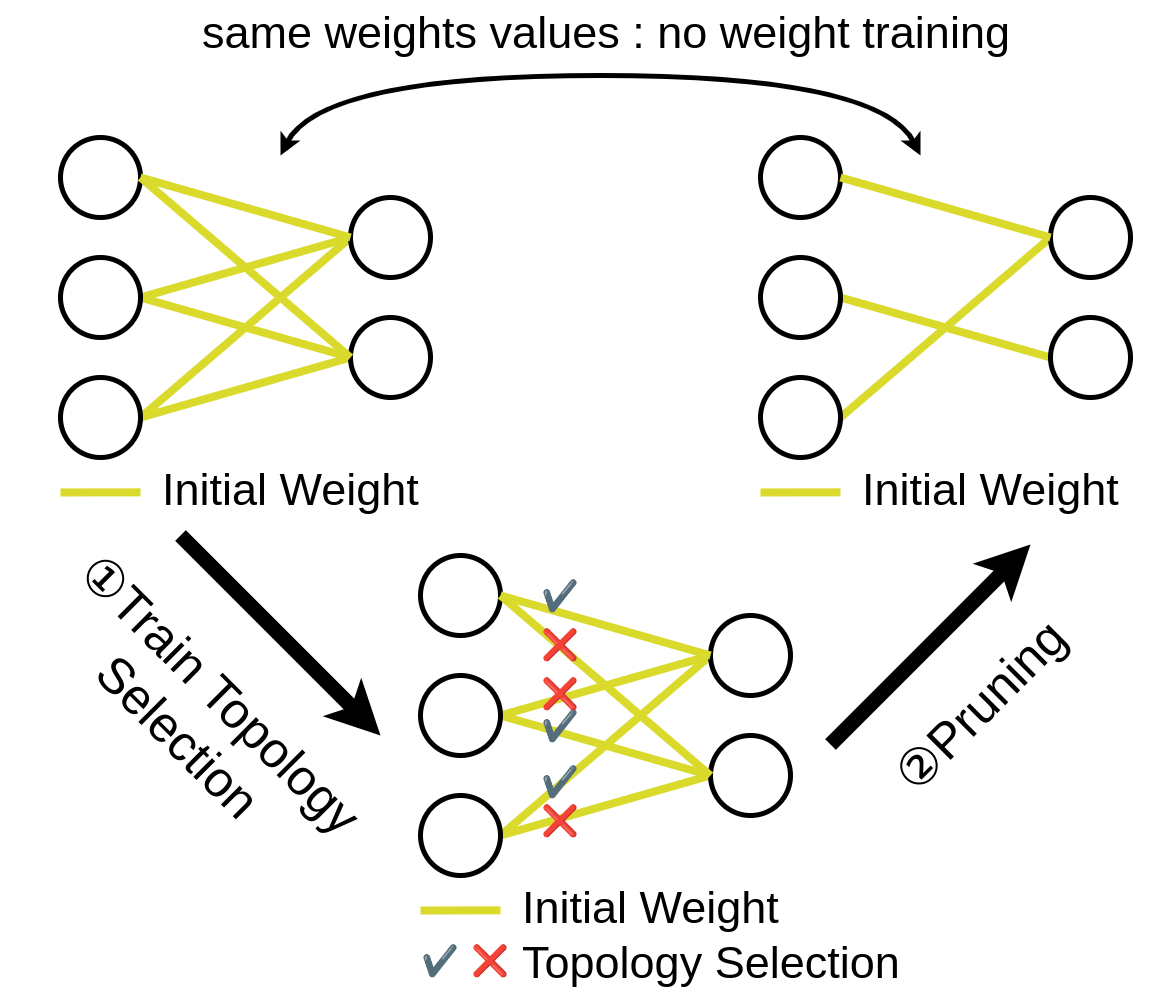
\includegraphics[width=0.4\textwidth]{chapter_2/assets/our_pruning_pipeline.png}}
  \vspace{0.10\textwidth}
  \subfloat[Standard pruning pipelines \label{fig:chap2:standard-pipeline}]{
    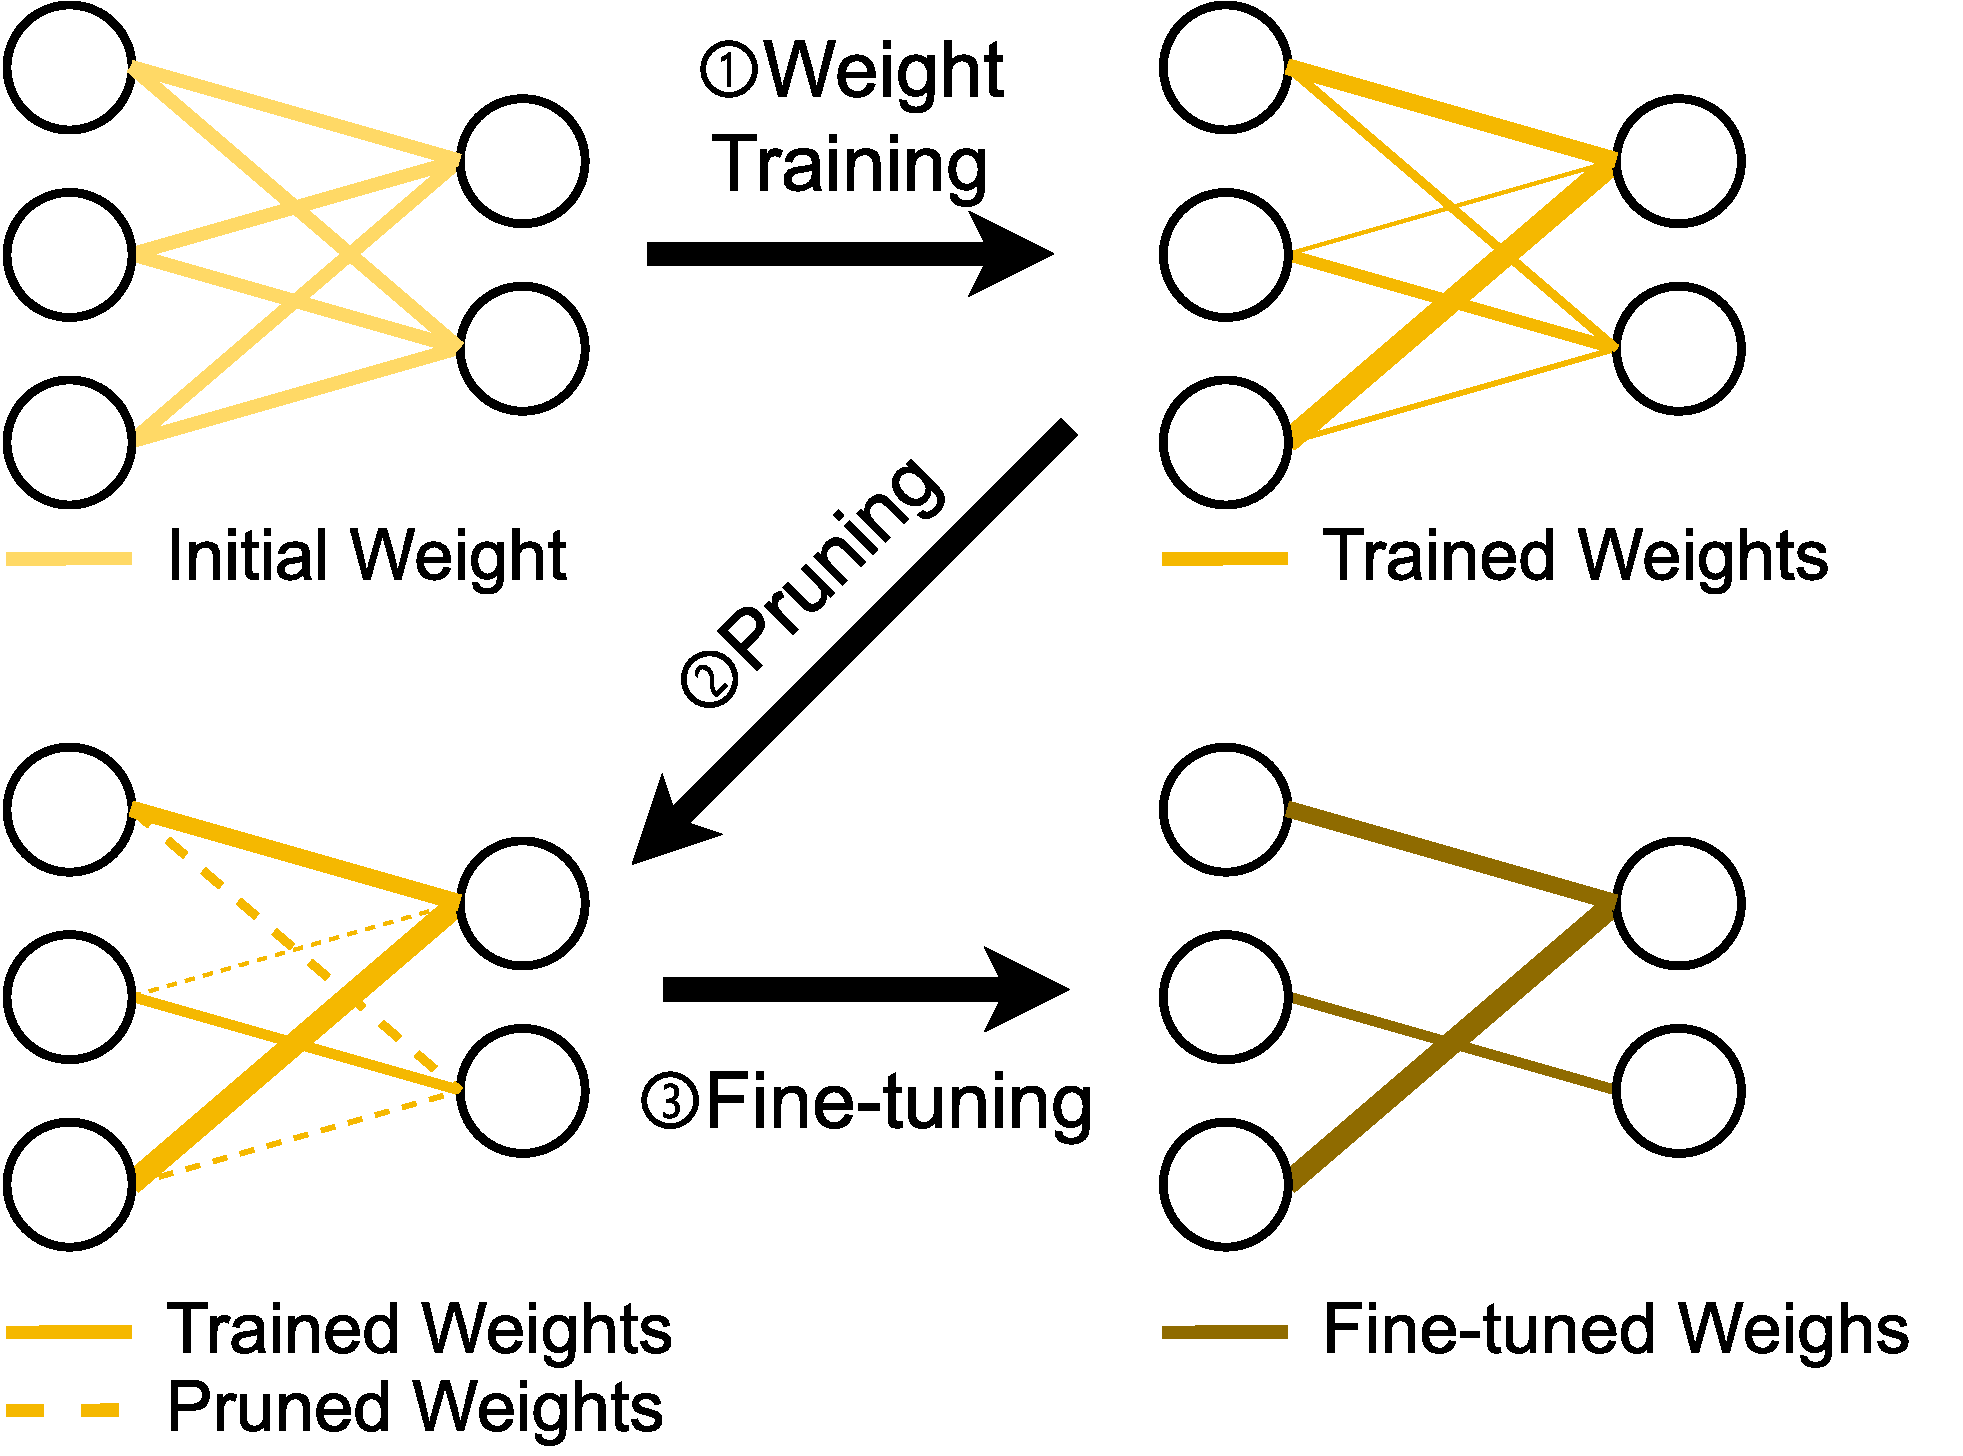
\includegraphics[width=0.4\textwidth]{chapter_2/assets/standard_pruning_pipeline.pdf}}
  \caption{Overview of our pruning pipeline and standard pruning pipelines.
    Our pipeline perfoms topology selection only: weights are not trained.
    On the contrary, standard pruning pipelines rely on weight training and fine-tuning.}
\end{figure}


\begin{algorithm}
  \caption{Our training procedure}
  \label{alg:chap2:ASLP}
  \begin{algorithmic}
    \REQUIRE Dataset $\mathcal{D} \subset \mathcal{X} \times \mathcal{Y}$, network $f$,
    weights $\theta$, latent masks $\bm{\hat{m}}$, number of epochs $n$, learning rate $\eta$
    \FOR{$t = 1$ to $n$}
    \FOR{each $(X,y) \in \mathcal{D}$}
    \STATE
    $q_{i,j} \gets \text{argmax}
      \begin{bmatrix}
        \bm{\hat{m}}_{i,j} + g_{i,j} \\
        0 + g'_{i,j}                 \\
      \end{bmatrix}$ \COMMENT{Sample of a topology}
    \STATE $m_{ij} \gets 1_{\{q_{ij}=1\}}$
    \COMMENT{Give the masks $\bm{m}_{i,j}$ their values}

    \STATE ${\cal L}\big(f_\theta(X,
        s_\ell (\bm{m}_\ell \odot \bm{w}_\ell)),y \big)$
    \COMMENT{Compute the loss with masked weights and \ac{SR}}
    \STATE $\bm{\hat{m}}_{t+1} = \bm{\hat{m}}_t - \eta \nabla_{\bm{\hat{m}}} \mathcal{L}$ \COMMENT{Backpropagate the loss and update the masks}
    \ENDFOR
    \ENDFOR
    \RETURN Network $f$ with unchanged weights $\theta$ and trained latent masks $\bm{\hat{m}}$.
  \end{algorithmic}
\end{algorithm}


\section{Experiments}
\label{sec:chap2:experiments}

In this section, we  evaluate the efficacy of our proposed method and we
investigate the influence of various parameters and configurations.
\Cref{sec:chap2:experimental_setup} details the experimental setups,
\cref{sec:chap2:performances} presents the performances of our method against
other state-of-the-art methods, namely Edge-popup
\cite{DBLP:conf/cvpr/RamanujanWKFR20} and Supermask
\cite{DBLP:conf/nips/ZhouLLY19}, both detailed in
\cref{sec:chap2:subnetwork_topology_extraction}.
\Cref{sec:chap2:validation_weight_rescaling} validates our weight-rescaling
strategy,  \cref{sec:chap2:impact_learning_rate} studies the impact of the
learning rate on the performance of our method, and validates our choice of
learning rate. Finally, \cref{sec:chap2:increasing_sparsity} investigates the
impact of imposing a fixed pruning rate after the training and presents
experimental results that support the effectiveness of our thresholding pruning
strategy method.


\subsection{Experimental Setup}
\label{sec:chap2:experimental_setup}

Our experiments were conducted on the CIFAR-10, CIFAR-100 and TinyImageNet
datasets which are described in \cref{sec:dlo:datasets}. Unless stated
otherwise, on each table we report the test accuracy evaluated on the test set
of the datasets. This accuracy is given in percentages with the standard
deviation. The latter is given numerically in tables or represented by the
shaded area around curves for figures. Each data point is obtained by averaging
5 independent runs. The architectures considered are Conv2, Conv4, Conv6, VGG16,
ResNet-20 and ResNet-18, which are presented in \cref{sec:dlo:architectures_used}\\

In order to demonstrate the efficacy of our method in a standard image
classification scenario, we compare our approach with state-of-the-art methods,
specifically Edge-popup \cite{DBLP:conf/cvpr/RamanujanWKFR20} and Supermask
\cite{DBLP:conf/nips/ZhouLLY19}. We re-implemented both methods in PyTorch
\cite{DBLP:conf/nips/PaszkeGMLBCKLGA19} and employed a uniform training
procedure for all methods: networks are trained for 1000 epochs with a fixed
learning rate of 50 (except for Edge-popup, which utilises a learning rate of
0.1). The learning rate of \ac{SR} is set to $10^{-3}$, and  neither weight
decay nor $\ell_2$ regularisation is applied. This section examines several
configurations initially presented in \cite{DBLP:conf/nips/ZhouLLY19}, which
encompass combinations of techniques or enhancements employed for method
evaluation. The various techniques include the application of \ac{WR}, the use
of \ac{SC} weight distribution
\cite{DBLP:conf/nips/ZhouLLY19,DBLP:conf/cvpr/RamanujanWKFR20} and data
augmentation.\\

\noindent\textbf{Weight Rescaling.} Each method discussed in this section
incorporates its own weight rescaling technique: \acf{DWR} for
\cite{DBLP:conf/nips/ZhouLLY19}, \acf{SKD} for
\cite{DBLP:conf/cvpr/RamanujanWKFR20} and \acf{SR} for \ac{ASLP} (Ours). All of
these techniques are denoted as \ac{WR} in this section. The three of them have
been detailed in \cref{sec:chap2:smart-rescale}\\

\noindent\textbf{Signed Constant Distribution.} The signed constant
distribution was introduced by \cite{DBLP:conf/nips/ZhouLLY19}. Weights sampled
from this distribution can take only two values: $-\sigma$ and $\sigma$, where
$\sigma$ represents the standard deviation of the weight tensor upon
initialization using the widely adopted Kaiming initialization
\cite{DBLP:conf/iccv/HeZRS15}, which is tailored to initialise weights in such a
way that the variance remains the same across every layer during both forward
and backward passes, especially for neural networks with \ac{ReLU} activation
functions (More details are given in \cref{sec:appendix:xavier_init}).
\citeauthor{DBLP:conf/nips/ZhouLLY19} report that it improves performances over
the standard weight initialisation scheme.\\

\noindent\textbf{Data augmentation.} Although
\citeauthor{DBLP:conf/nips/ZhouLLY19} \cite{DBLP:conf/nips/ZhouLLY19} did not
used any data augmentation, it is a widely accepted practice in image
classification and is generally applied even if not explicitly mentioned by the
authors (for example \citeauthor{DBLP:conf/cvpr/RamanujanWKFR20} used data
augmentation in their code \cite{hidden-networks} altough it is not mentioned in
the original article \cite{DBLP:conf/cvpr/RamanujanWKFR20}). Consequently, we
consider two configurations: with and without data augmentation. The data
augmentation we apply has been observed in various state-of-the-art
implementations
\cite{hidden-networks,openlth_dataaugmentation,rethinking_dataaugmentatino} and
is the following: first, images are padded with zeroes, next, a random crop of
the original size is extracted from the padded image. Lastly, a random
horizontal flip is performed. An example of this data augmentation pipeline is
displayed in \cref{fig:chap2:data_augmentation_pipeline}.\\

\begin{figure}[h!]
  \centering
  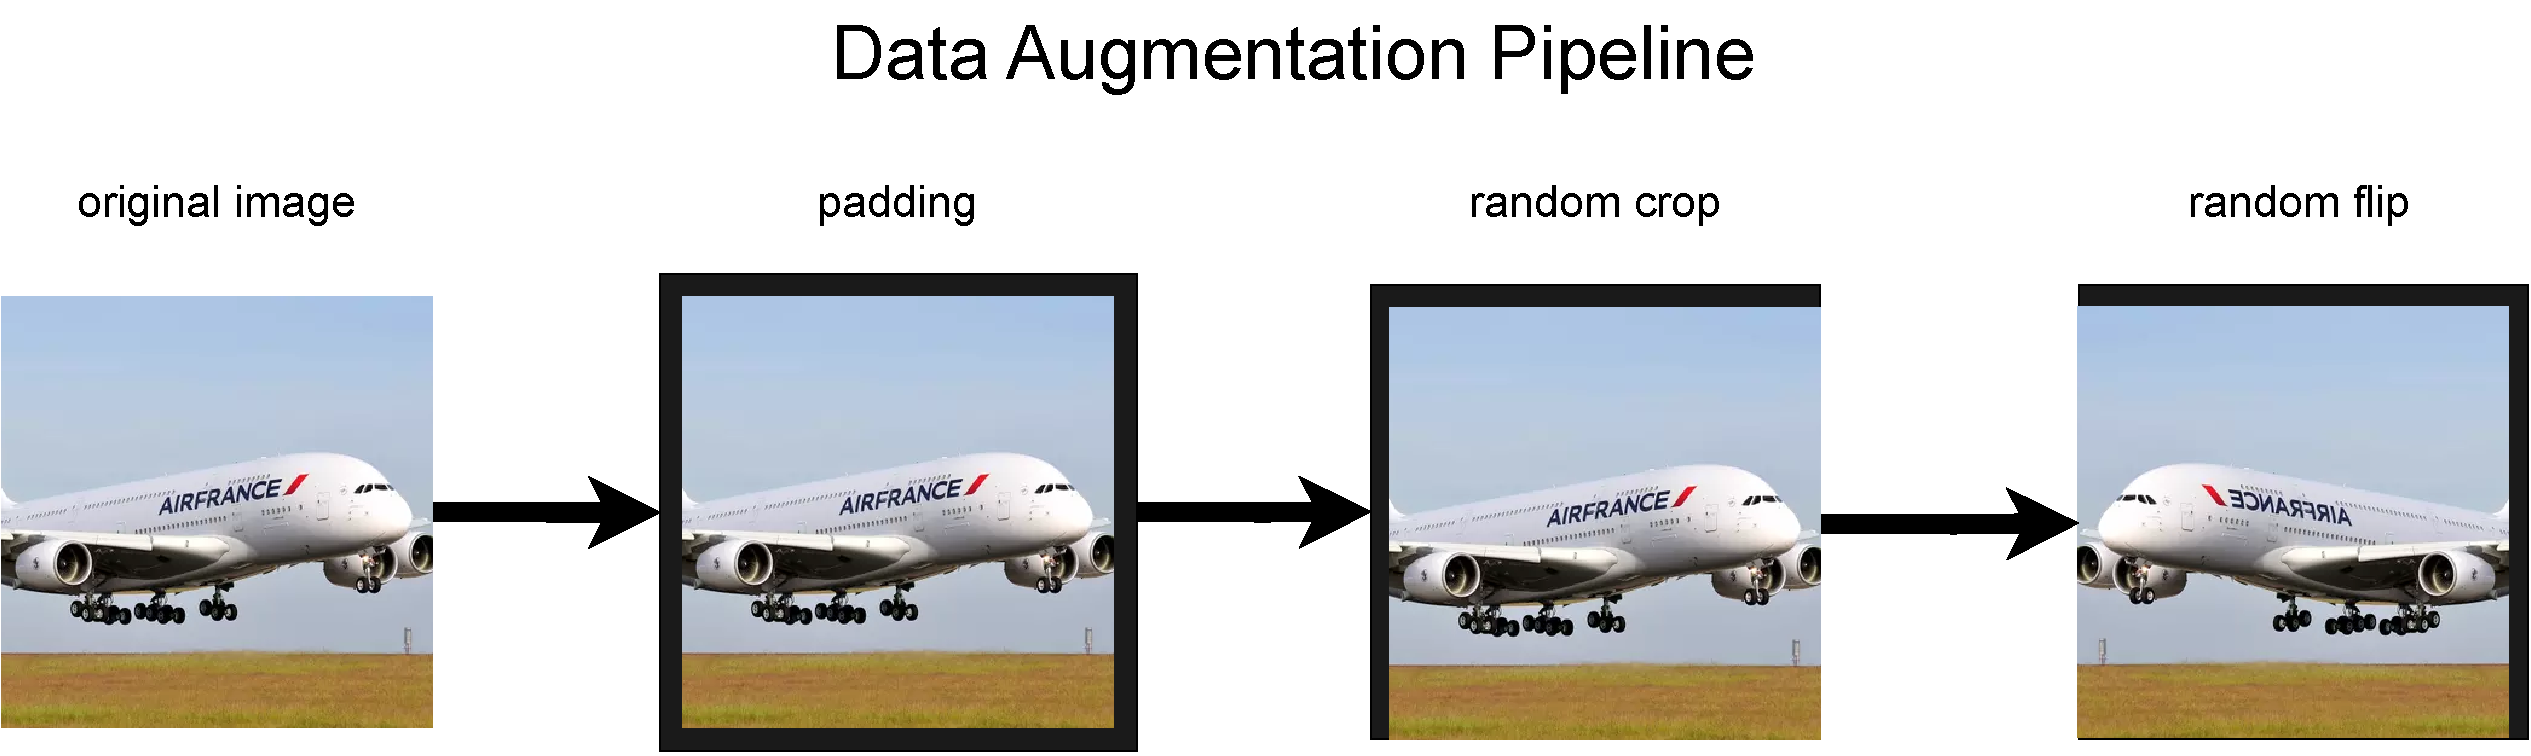
\includegraphics[width=0.8\textwidth]{chapter_2/assets/data_augmentation_pipeline.pdf}
  \caption{Data Augmentation pipeleine example used for CIFAR-10 and CIFAR-100.}
  \label{fig:chap2:data_augmentation_pipeline}
\end{figure}

\noindent\textbf{Pruning Strategy.} To prune the networks trained with our
method, we chose to freeze the topology with our \emph{threhsolding} pruning
strategy, described in \cref{sec:chap2:freezing_topology}, which thresholds the
probabilities of selection $p_{ij}$ and consequently the latent masks
$\bm{\hat{m}}_{ij}$. As a matter of comparison, we also consider the setting in
\cite{DBLP:conf/nips/ZhouLLY19} which is an averaging strategy to evaluate
Supermask performance. It consists in sampling ten different topologies,
yielding effectively 10 different subnetworks. The performances of each of these
subnetworks are evaluated independently giving 10 test accuracies that are
averaged to obtain the final test accuracy. We refer to this pruning strategy as
\textit{averaging}. In the Edge-popup method
\cite{DBLP:conf/cvpr/RamanujanWKFR20}, described in
\cref{sec:chap2:subnetwork_topology_extraction}, the pruning rate (denoted $k$
by the authors) is inherently incorporated with two primary characteristics:
$\emph{(i)}$ the set of pruned weights is deterministic (the pruned weights are
the ones associated with the bottom-k saliency indicators), and $\emph{(ii)}$
the fraction of pruned weights is strictly equal to the predetermined pruning
rate. As a result, a distinct pruning step enforcing the predetermined pruning
rate is redundant since it would not bring any changes to the network structure
or the values of the weights.\\

\subsection{Performances}
\label{sec:chap2:performances}

Overall, the analysis of our \ac{ASLP} method results, presented in
\cref{tab:chap2:con_performances_comparison_cifar10,tab:chap2:con_performances_comparison_cifar100,tab:chap2:r20_VGG16_performances_comparison,tab:chap2:tinyimagenet_performances_comparison},
shows that \ac{ASLP} outperforms both Edge Popup and Supermask methods on
CIFAR-10 and CIFAR-100 datasets, a trend consistent across all tested networks,
including Conv2, Conv4, Conv6, VGG16, and ResNet20. Notably, our
\textit{thresholding} pruning strategy demonstrated superior performance
compared to Supermask \textit{averaging} approach (see
\cref{sec:chap2:freezing_topology} for details of both strategies). The
\textit{thresholding} strategy ensures that the most likely-to-be-selected
weights are incorporated into the final frozen network. It is accomplished by
setting a threshold on $p_{ij}$, the probability for a weight of being selected.
Only those weights exceeding this threshold are preserved, leading to the
retention of most valuable connections in the network. This approach focuses on
the utilisation of high impact weights, which contributes to the enhanced
performance of the pruned network. Contrastingly, the \textit{averaging}
strategy employed by the Supermask method \cite{DBLP:conf/nips/ZhouLLY19} takes
a different approach. It draws 10 random subnetworks, each possessing a distinct
set of weights. However, this strategy introduces a risk, as these randomly
selected weight sets may contain weights that contribute minimally to the
network overall performance. The inclusion of such potentially useless weights
could reduce the performance of the pruned network.\\

Remarkably, for larger networks such as VGG16 and ResNet-20, our \ac{ASLP}
method employing the \textit{thresholding} strategy also consistently surpasses
all other methods (see \cref{tab:chap2:r20_VGG16_performances_comparison}).
Nevertheless, a ResNet-18 trained on TinyImagenet with \ac{ASLP} is outperformed
by its counterpart trained with Edge-popup (see
\cref{tab:chap2:tinyimagenet_performances_comparison}).\\

We put forth several hypotheses to account for the reduced performance. First,
the ResNet-18 architecture employed is the standard PyTorch implementation
\cite{pytorch_resnet18}, designed for the ImageNet dataset
\cite{deng2009imagenet}. As a result, it is tailored for $224 \times 224$ pixel
images, while TinyImageNet images are only $64 \times 64$ pixels. With a smaller
input image size, each pixel encompasses a larger area of the input space, and
an overly large receptive field for a smaller image like TinyImageNet may lead
to the loss of crucial spatial information. We opted against upscaling
TinyImageNet images to $224 \times 224$ as a preprocessing step in order to
prevent an exponential increase in computational cost.\\

Secondly, the ResNet-18 network is among the largest networks we examined,
having roughly 3 times the number of parameters of a Conv4 network (refer to
\cref{tab:dlo:networks_size}). As a result, there are numerous possible weight
combinations and subnetworks. Viewing \ac{ASLP} as a Neural Architecture Search
method, the search space for ResNet-18 is considerably larger than for the
Conv\{2,4,6\} networks. Nevertheless, the number of sampled topologies is only
equal to the product of the number of batches and the number of epochs during
which the network is trained. \Cref{tab:chap2:topologies_exploration} presents
the details of 2 setups: ResNet-18 trained on TinyImageNet and Conv4 trained on
CIFAR-10. It shows that the fraction of explored topologies by our \ac{ASLP}
method, is considerably higher for the Conv4 network than for the ResNet-18 one
in the given configurations. The number of explored topologies might be
sufficient to sweep the search space for Conv\{2,4,6\} networks and find a
compelling and effective subnetwork, but it might not be enough for a ResNet-18
network.\\

\begin{table}
  \centering
  \resizebox{\textwidth}{!}{
    \begin{tabular}{lcc}
      \cmidrule[\heavyrulewidth]{2-3}
                                                         & \textbf{Conv4 \&
        CIFAR-10}
                                                         &
      \textbf{ ResNet-18 \& TinyImageNet}
      \\
      \midrule
      Number of parameters ($N$)                         & 2,425,930                            & 11,685,608 \\
      Train Dataset Size (number or images)              & 50,000                               & 90,000     \\
      Batch Size used for training                       & 256                                  & 256        \\
      Nb. of batches for 1 epoch                         & 196                                  & 352        \\
      Nb. of explored topologies in $10^3$ epochs ($E$)  & 196,000                              & 352,000    \\
      Nb. of possible topologies ($P$)                   & $P=2^N \approx
      5\times 10^{10^{5.86}}$                    & $P=2^N \approx 5\times
      10^{10^{6.54}}$              \\
      Fraction of explored topologies ($\nu_\text{exp}$) &
      $\nu_\text{exp}^\text{Conv4} = \displaystyle\frac{E}{P} \approx
      10^{{-10}^{5.86}}$                                 & $\nu_\text{exp}^\text{ResNet-18} =
      \displaystyle\frac{E}{P} \approx 10^{{-10}^{6.54}}$                                                    \\
      Ratio of fraction of explored topologies           &
      \multicolumn{2}{c}{$\displaystyle\frac{\nu_\text{exp}^\text{Conv4}}{\nu_\text{exp}^\text{ResNet-18}}
      \approx 10^{10^{6.44}}$}                                                                               \\
      \bottomrule
    \end{tabular}
  } \caption {Comparison of the number of explored topologies for the Conv4 and
    ResNet-18 networks with CIFAR-10 and TinyImageNet, respectively. Since a new
    topology is sampled for every batch, the number of explored topologies ($E$)
    is computed as the product of the number of batches and the number of epochs
    during which the network is trained (here $10^3$). The number of possible
    topologies ($P$) is computed as the number of possible weight combinations
    in the network ($2^N$). The fraction of explored topologies is computed as
    the ratio of the fraction of explored topologies for the Conv4 network and
    the fraction of explored topologies for the ResNet-18 network. In these
    experimental setups, the fraction of explored topologies for the Conv4
    network significantly higher than the fraction of explored topologies for
    the ResNet-18 network.}
  \label{tab:chap2:topologies_exploration}
\end{table}


However, this hypothesis warrants further clarification. Indeed, the VGG16
network has more parameters than the ResNet-18 (see
\cref{tab:dlo:networks_size}), nevertheles, in our experiments, \ac{ASLP}
achieves superior results compared to other methods on the VGG16 architecture.
We suggest the following explanation: First, the CIFAR-10 and CIFAR-100 datasets
are simpler datasets with less classes, compared to TinyImageNet. Secondly,
although the VGG16 has more parameters, it has fewer weights in its fully
connected layers since the datasets it is benchmarked on have fewer classes.
Indeed, a VGG16 network tailored for CIFAR-100 has 51,200 parameters in its last
fully connected layer, whereas a ResNet-18 network designed for TinyImageNet has
102,400. Thus, the search space for the fully connected part of the VGG network
is significantly smaller than on the ResNet-18 network. Therefore, because of
the smaller search space, \ac{ASLP} founds a more optimal subset of weights for
the last layer of the VGG16 network than the ResNet-18 one. This final fully
connected layer of a neural network plays a crucial role in determining its
overall performance and accuracy in predicting outcomes.\\

%=============================================




% region: perf-tables


\begin{table}[htbp]
  \centering

  \begin{subtable}[t]{\textwidth}
    \centering
    \resizebox{14cm}{!}{
      \begin{tabular}{llcccc}
        \cmidrule[\heavyrulewidth]{3-6}
                                                           &                                                  & $\varnothing$             & \textbf{SC}               & \textbf{WR}               & \textbf{WR+SC}            \\
        \toprule
        % Conv 2 results
        \multirow{12}{*}{} \multirow{4}{*}{\textbf{Conv2}} & \ac{ASLP} (thresholding)                              & \textbf{75.70 $\pm$ 0.30} & \textbf{75.81 $\pm$ 0.69} & \textbf{76.48 $\pm$ 0.68} & \textbf{76.92 $\pm$ 0.24} \\
                                                           & \ac{ASLP} (averaging)                                 & 75.42 $\pm$ 0.25          & 75.50 $\pm$ 0.56          & 76.05 $\pm$ 0.44          & 76.44 $\pm$ 0.19          \\
                                                           & \cite{DBLP:conf/nips/ZhouLLY19} (averaging)      & -                         & -                         & -                         & -                         \\
                                                           & \cite{DBLP:conf/cvpr/RamanujanWKFR20} ($k=50\%$) & 74.18 $\pm$ 0.76          & 75.19 $\pm$ 0.56          & 74.51 $\pm$ 0.31          & 75.45 $\pm$ 0.44          \\
        \midrule
        % Conv 4 results
        \multirow{4}{*}{\textbf{Conv4}}                    & \ac{ASLP} (thresholding)                              & \textbf{83.03 $\pm$ 0.31} & \textbf{83.73 $\pm$ 0.46} & \textbf{83.59 $\pm$ 0.29} & \textbf{84.06 $\pm$ 0.31} \\
                                                           & \ac{ASLP} (averaging)                                 & 82.29 $\pm$ 0.25          & 83.22 $\pm$ 0.56          & 82.79 $\pm$ 0.30          & 83.46 $\pm$ 0.49          \\
                                                           & \cite{DBLP:conf/nips/ZhouLLY19} (averaging)      & -                         & -                         & -                         & -                         \\
                                                           & \cite{DBLP:conf/cvpr/RamanujanWKFR20} ($k=50\%$) & 82.38 $\pm$ 0.29          & 83.61 $\pm$ 0.38          & 81.71 $\pm$ 0.59          & 83.55 $\pm$ 0.32          \\
        \midrule
        % Conv 6 results
        \multirow{4}{*}{\textbf{Conv6}}                    & \ac{ASLP} (thresholding)                              & \textbf{84.98 $\pm$ 0.33} & \textbf{86.49 $\pm$ 0.36} & \textbf{85.32 $\pm$ 0.27} & \textbf{86.21 $\pm$ 0.34} \\
                                                           & \ac{ASLP} (averaging)                                 & 84.24 $\pm$ 0.28          & 85.67 $\pm$ 0.34          & 84.51 $\pm$ 0.35          & 85.49 $\pm$ 0.38          \\
                                                           & \cite{DBLP:conf/nips/ZhouLLY19} (averaging)      & -                         & -                         & -                         & -                         \\
                                                           & \cite{DBLP:conf/cvpr/RamanujanWKFR20} ($k=50\%$) & 84.67 $\pm$ 0.35          & 85.87 $\pm$ 0.13          & 84.37 $\pm$ 0.58          & 85.84 $\pm$ 0.51          \\
        \bottomrule
      \end{tabular}
    }
    \caption{With data augmentation.}
    \label{tab:chap2:perf-tables:with-augmentation}
  \end{subtable}

  \bigskip

  \begin{subtable}[t]{\textwidth}
    \centering
    \resizebox{14cm}{!}{
      \begin{tabular}{llcccc}
        \cmidrule[\heavyrulewidth]{3-6}
                                                           &                                                  & $\varnothing$             & \textbf{SC}                & \textbf{WR}               & \textbf{WR+SC}            \\
        \toprule
        % Conv 2 results
        \multirow{12}{*}{} \multirow{4}{*}{\textbf{Conv2}} & \ac{ASLP} (thresholding)                              & \textbf{68.24 $\pm$ 0.14} & \textbf{ 68.11 $\pm$ 0.64} & \textbf{66.84 $\pm$ 0.46} & \textbf{66.05 $\pm$ 0.93} \\
                                                           & \ac{ASLP} (averaging)                                 & 68.09 $\pm$ 0.35          & 67.69 $\pm$ 0.52           & 65.79 $\pm$ 0.65          & 65.35 $\pm$ 0.83          \\
                                                           & \cite{DBLP:conf/nips/ZhouLLY19} (averaging)      & 67.12 $\pm$ 0.25          & 66.34 $\pm$ 0.41           & 56.71 $\pm$ 2.99          & 56.26 $\pm$ 1.64          \\
                                                           & \cite{DBLP:conf/cvpr/RamanujanWKFR20} ($k=50\%$) & -                         & -                          & -                         & -                         \\
        \midrule
        % Conv 4 results
        \multirow{4}{*}{\textbf{Conv4}}                    & \ac{ASLP} (thresholding)                              & \textbf{71.64 $\pm$ 0.36} & \textbf{69.74 $\pm$ 1.37}  & \textbf{72.85 $\pm$ 0.48} & \textbf{72.08 $\pm$ 0.62} \\
                                                           & \ac{ASLP} (averaging)                                 & 70.88 $\pm$ 0.47          & 68.77 $\pm$ 1.42           & 71.82 $\pm$ 0.53          & 71.09 $\pm$ 0.69          \\
                                                           & \cite{DBLP:conf/nips/ZhouLLY19} (averaging)      & 68.09 $\pm$ 0.84          & 67.48 $\pm$ 0.52           & 58.13 $\pm$ 2.39          & 53.84 $\pm$ 5.00          \\
                                                           & \cite{DBLP:conf/cvpr/RamanujanWKFR20} ($k=50\%$) & -                         & -                          & -                         & -                         \\
        \midrule
        % Conv 6 results
        \multirow{4}{*}{\textbf{Conv6}}                    & \ac{ASLP} (thresholding)                              & \textbf{73.32 $\pm$ 0.42} & \textbf{69.83 $\pm$ 1.46}  & \textbf{76.20 $\pm$ 0.91} & \textbf{75.30 $\pm$ 0.89} \\
                                                           & \ac{ASLP} (averaging)                                 & 72.62 $\pm$ 0.57          & 69.53 $\pm$ 1.68           & 75.24 $\pm$ 0.69          & 74.50 $\pm$ 0.96          \\
                                                           & \cite{DBLP:conf/nips/ZhouLLY19} (averaging)      & 70.71 $\pm$ 0.98          & 69.16 $\pm$ 1.92           & 44.77 $\pm$ 17.02         & 36.59 $\pm$ 15.32         \\
                                                           & \cite{DBLP:conf/cvpr/RamanujanWKFR20} ($k=50\%$) & -                         & -                          & -                         & -                         \\
        \bottomrule
      \end{tabular}
    }
    \caption{Without data augmentation.}
    \label{tab:chap2:perf-tables:without-augmentation}
  \end{subtable}
  \caption{Comparison of \ac{ASLP} \textbf{test accuracy} against Edge-Popup and
    Supermask \cite{DBLP:conf/cvpr/RamanujanWKFR20,DBLP:conf/nips/ZhouLLY19} on
    \textbf{CIFAR-10} using various configurations. We reimplemented the
    configurations tested by the authors in their articles. Performances are
    presented with (\cref{tab:chap2:perf-tables:with-augmentation}) and without
    (\cref{tab:chap2:perf-tables:without-augmentation}) data augmentation,
    \acf{WR}, and \acf{SC} weight distribution. A dash denotes a configuration
    that was not tested by the authors. Our method performances are reported for
    both the \textit{thresholding} and \textit{averaging} setups detailed in
    \cref{sec:chap2:freezing_topology}. For Edge-popup, we use the value of $k$
    which yeilds the best test accuracy for Conv\{2,4,6\}, as reported in
    \cite{DBLP:conf/cvpr/RamanujanWKFR20}. Across all setups, our method ASLP
    outperforms Edge-Popup and Supermask.}
  \label{tab:chap2:con_performances_comparison_cifar10}

\end{table}


% \begin{table}[htbp]
%   \centering
%   \resizebox{16.5cm}{!} {
%     \begin{tabular}{llcccccccc}
%       \cmidrule[\heavyrulewidth]{3-10}
%                                                          &                                                  & \multicolumn{4}{c}{\textbf{w/ data augmentation}} & \multicolumn{4}{c}{\textbf{w/o augmentation}}                                                                                                                                                                          \\
%                                                          &                                                  & $\varnothing$                                     & \textbf{SC}                                   & \textbf{WR}               & \textbf{WR+SC}            & $\varnothing$             & \textbf{SC}                & \textbf{WR}               & \textbf{WR+SC}            \\
%       \toprule

%       % Conv 2 results
%       \multirow{12}{*}{} \multirow{4}{*}{\textbf{Conv2}} & \ac{ASLP} (thresholding)                              & \textbf{75.70 $\pm$ 0.30}                         & \textbf{75.81 $\pm$ 0.69}                     & \textbf{76.48 $\pm$ 0.68} & \textbf{76.92 $\pm$ 0.24} & \textbf{68.24 $\pm$ 0.14} & \textbf{ 68.11 $\pm$ 0.64} & \textbf{66.84 $\pm$ 0.46} & \textbf{66.05 $\pm$ 0.93} \\
%                                                          & \ac{ASLP} (averaging)                                 & 75.42 $\pm$ 0.25                                  & 75.50 $\pm$ 0.56                              & 76.05 $\pm$ 0.44          & 76.44 $\pm$ 0.19          & 68.09 $\pm$ 0.35          & 67.69 $\pm$ 0.52           & 65.79 $\pm$ 0.65          & 65.35 $\pm$ 0.83          \\
%                                                          & \cite{DBLP:conf/nips/ZhouLLY19} (averaging)      & -                                                 & -                                             & -                         & -                         & 67.12 $\pm$ 0.25          & 66.34 $\pm$ 0.41           & 56.71 $\pm$ 2.99          & 56.26 $\pm$ 1.64          \\
%                                                          & \cite{DBLP:conf/cvpr/RamanujanWKFR20} ($k=50\%$) & 74.18 $\pm$ 0.76                                  & 75.19 $\pm$ 0.56                              & 74.51 $\pm$ 0.31          & 75.45 $\pm$ 0.44          & -                         & -                          & -                         & -                         \\
%       \midrule

%       % Conv 4 results
%       \multirow{4}{*}{\textbf{Conv4}}                    & \ac{ASLP} (thresholding)                              & \textbf{83.03 $\pm$ 0.31}                         & \textbf{83.73 $\pm$ 0.46}                     & \textbf{83.59 $\pm$ 0.29} & \textbf{84.06 $\pm$ 0.31} & \textbf{71.64 $\pm$ 0.36} & \textbf{69.74 $\pm$ 1.37}  & \textbf{72.85 $\pm$ 0.48} & \textbf{72.08 $\pm$ 0.62} \\
%                                                          & \ac{ASLP} (averaging)                                 & 82.29 $\pm$ 0.25                                  & 83.22 $\pm$ 0.56                              & 82.79 $\pm$ 0.30          & 83.46 $\pm$ 0.49          & 70.88 $\pm$ 0.47          & 68.77 $\pm$ 1.42           & 71.82 $\pm$ 0.53          & 71.09 $\pm$ 0.69          \\
%                                                          & \cite{DBLP:conf/nips/ZhouLLY19} (averaging)      & -                                                 & -                                             & -                         & -                         & 68.09 $\pm$ 0.84          & 67.48 $\pm$ 0.52           & 58.13 $\pm$ 2.39          & 53.84 $\pm$ 5.00          \\
%                                                          & \cite{DBLP:conf/cvpr/RamanujanWKFR20} ($k=50\%$) & 82.38 $\pm$ 0.29                                  & 83.61 $\pm$ 0.38                              & 81.71 $\pm$ 0.59          & 83.55 $\pm$ 0.32          & -                         & -                          & -                         & -                         \\
%       \midrule

%       % Conv 6 results
%       \multirow{4}{*}{\textbf{Conv6}}                    & \ac{ASLP} (thresholding)                              & \textbf{84.98 $\pm$ 0.33}                         & \textbf{86.49 $\pm$ 0.36}                     & \textbf{85.32 $\pm$ 0.27} & \textbf{86.21 $\pm$ 0.34} & \textbf{73.32 $\pm$ 0.42} & \textbf{69.83 $\pm$ 1.46}  & \textbf{76.20 $\pm$ 0.91} & \textbf{75.30 $\pm$ 0.89} \\
%                                                          & \ac{ASLP} (averaging)                                 & 84.24 $\pm$ 0.28                                  & 85.67 $\pm$ 0.34                              & 84.51 $\pm$ 0.35          & 85.49 $\pm$ 0.38          & 72.62 $\pm$ 0.57          & 69.53 $\pm$ 1.68           & 75.24 $\pm$ 0.69          & 74.50 $\pm$ 0.96          \\
%                                                          & \cite{DBLP:conf/nips/ZhouLLY19} (averaging)      & -                                                 & -                                             & -                         & -                         & 70.71 $\pm$ 0.98          & 69.16 $\pm$ 1.92           & 44.77 $\pm$ 17.02         & 36.59 $\pm$ 15.32         \\
%                                                          & \cite{DBLP:conf/cvpr/RamanujanWKFR20} ($k=50\%$) & 84.67 $\pm$ 0.35                                  & 85.87 $\pm$ 0.13                              & 84.37 $\pm$ 0.58          & 85.84 $\pm$ 0.51          & -                         & -                          & -                         & -                         \\
%       \bottomrule
%     \end{tabular}
%   }
%   \caption{\textbf{OLD TABLE} Comparison of \ac{ASLP} performance against Edge-Popup and Supermask
%     \cite{DBLP:conf/cvpr/RamanujanWKFR20,DBLP:conf/nips/ZhouLLY19} on CIFAR-10
%     using various configurations. We use the configurations tested by the author
%     of the aforementioned articles. Performance measures reported are accuracy and
%     are presented with and without data augmentation, weight rescaling (WR), and
%     the signed constant weight distribution (SC). We report performances for both
%     \textit{thresholding} and \textit{averaging} setups for our method. For edge-popup, we use
%     the best $k$ value for Conv\{2,4,6\} reported in
%     \cite{DBLP:conf/cvpr/RamanujanWKFR20}.  Across all setups, our method ASLP
%     outperforms Edge-Popup and Supermask}
%   \label{tab:chap2:con_performances_comparison_cifar10_vold}

% \end{table}


\begin{table}[htbp]
  \centering
  \begin{subtable}[t]{\textwidth}
    \centering
    \resizebox{14cm}{!}{
      \begin{tabular}{llllll}
        \cmidrule[\heavyrulewidth]{3-6}
                                        &                                                  & $\varnothing$             & \textbf{SC}               & \textbf{WR}               & \textbf{WR+SC}            \\
        \toprule
        \multirow{12}{*}{}
        \multirow{4}{*}{\textbf{Conv2}} & \ac{ASLP} (thresholding)                              & \textbf{38.64 $\pm$ 0.92} & 38.31 $\pm$ 0.75          & \textbf{41.81 $\pm$ 0.84} & \textbf{42.06 $\pm$ 0.76} \\
                                        & \ac{ASLP} (averaging)                                 & 38.49 $\pm$ 0.61          & 38.18 $\pm$ 0.81          & 41.12 $\pm$ 0.66          & 41.17 $\pm$ 0.54          \\
                                        & \cite{DBLP:conf/nips/ZhouLLY19} (averaging)      & -                         & -                         & -                         & -                         \\
                                        & \cite{DBLP:conf/cvpr/RamanujanWKFR20} ($k=50\%$) & 38.47 $\pm$ 0.46          & \textbf{39.83 $\pm$ 0.46} & 38.57 $\pm$ 0.59          & 39.87 $\pm$ 0.78          \\
        \midrule

        \multirow{4}{*}{\textbf{Conv4}} & \ac{ASLP} (thresholding)                              & \textbf{47.78 $\pm$ 1.18} & 49.33 $\pm$ 0.77          & \textbf{50.33 $\pm$ 0.39} & \textbf{51.49 $\pm$ 0.43} \\
                                        & \ac{ASLP} (averaging)                                 & 47.18 $\pm$ 1.17          & 48.78 $\pm$ 0.79          & 49.39 $\pm$ 0.30          & 50.17 $\pm$ 0.50          \\
                                        & \cite{DBLP:conf/nips/ZhouLLY19} (averaging)      & -                         & -                         & -                         & -                         \\
                                        & \cite{DBLP:conf/cvpr/RamanujanWKFR20} ($k=50\%$) & 47.75 $\pm$ 0.63          & \textbf{50.16 $\pm$ 0.47} & 48.20 $\pm$ 0.72          & 50.02 $\pm$ 0.65          \\
        \midrule

        \multirow{4}{*}{\textbf{Conv6}} & \ac{ASLP} (thresholding)                              & 51.09 $\pm$ 0.92          & 53.00 $\pm$ 0.52          & \textbf{51.70 $\pm$ 0.48} & 52.85 $\pm$ 0.50          \\
                                        & \ac{ASLP} (averaging)                                 & 50.22 $\pm$ 1.09          & 51.72 $\pm$ 0.73          & 50.56 $\pm$ 0.33          & 51.59 $\pm$ 0.24          \\
                                        & \cite{DBLP:conf/nips/ZhouLLY19} (averaging)      & -                         & -                         & -                         & -                         \\
                                        & \cite{DBLP:conf/cvpr/RamanujanWKFR20} ($k=50\%$) & \textbf{51.13 $\pm$ 0.39} & \textbf{53.48 $\pm$ 0.51} & 51.06 $\pm$ 1.11          & \textbf{54.01 $\pm$ 0.35} \\
        \bottomrule
      \end{tabular}
    }
    \caption{With data augmentation}
  \end{subtable}

  \bigskip

  \begin{subtable}[t]{\textwidth}
    \centering
    \resizebox{14cm}{!}{
      \begin{tabular}{llllll}
        \cmidrule[\heavyrulewidth]{3-6}
                                        &                                                  & $\varnothing$             & \textbf{SC}               & \textbf{WR}               & \textbf{WR+SC}            \\
        \toprule
        \multirow{12}{*}{}
        \multirow{4}{*}{\textbf{Conv2}} & \ac{ASLP} (thresholding)                              & \textbf{38.72 $\pm$ 0.59} & 38.64 $\pm$ 1.23          & \textbf{42.42 $\pm$ 0.30} & \textbf{41.95 $\pm$ 0.68} \\
                                        & \ac{ASLP} (averaging)                                 & 38.40 $\pm$ 0.81          & \textbf{38.71 $\pm$ 1.05} & 41.66 $\pm$ 0.39          & 41.42 $\pm$ 0.55          \\
                                        & \cite{DBLP:conf/nips/ZhouLLY19} (averaging)      & 38.09 $\pm$ 1.03          & 37.28 $\pm$ 0.47          & 26.03 $\pm$ 2.23          & 23.49 $\pm$ 1.36          \\
                                        & \cite{DBLP:conf/cvpr/RamanujanWKFR20} ($k=50\%$) & -                         & -                         & -                         & -                         \\
        \midrule

        \multirow{4}{*}{\textbf{Conv4}} & \ac{ASLP} (thresholding)                              & \textbf{47.56 $\pm$ 0.36} & \textbf{49.30 $\pm$ 0.54} & \textbf{50.39 $\pm$ 0.58} & \textbf{51.16 $\pm$ 0.94} \\
                                        & \ac{ASLP} (averaging)                                 & 46.89 $\pm$ 0.52          & 48.74 $\pm$ 0.47          & 49.55 $\pm$ 0.57          & 50.23 $\pm$ 0.87          \\
                                        & \cite{DBLP:conf/nips/ZhouLLY19} (averaging)      & 45.84 $\pm$ 1.01          & 47.72 $\pm$ 0.75          & 27.70 $\pm$ 2.41          & 27.53 $\pm$ 5.20          \\
                                        & \cite{DBLP:conf/cvpr/RamanujanWKFR20} ($k=50\%$) & -                         & -                         & -                         & -                         \\

        \midrule

        \multirow{4}{*}{\textbf{Conv6}} & \ac{ASLP} (thresholding)                              & \textbf{51.43 $\pm$ 0.41} & \textbf{53.10 $\pm$ 0.27} & \textbf{51.52 $\pm$ 0.35} & \textbf{53.22 $\pm$ 0.54} \\
                                        & \ac{ASLP} (averaging)                                 & 50.47 $\pm$ 0.42          & 52.00 $\pm$ 0.27          & 50.38 $\pm$ 0.33          & 51.82 $\pm$ 0.34          \\
                                        & \cite{DBLP:conf/nips/ZhouLLY19} (averaging)      & 49.19 $\pm$ 0.75          & 50.66 $\pm$ 0.47          & 2.54 $\pm$ 1.63           & 9.21 $\pm$ 5.50           \\
                                        & \cite{DBLP:conf/cvpr/RamanujanWKFR20} ($k=50\%$) & -                         & -                         & -                         & -                         \\

        \bottomrule
      \end{tabular}
    }
    \caption{Without data augmentation}
  \end{subtable}

  \caption{Comparison of \ac{ASLP} \textbf{test accuracy} against Edge-Popup and Supermask
    \cite{DBLP:conf/cvpr/RamanujanWKFR20,DBLP:conf/nips/ZhouLLY19} on \textbf{CIFAR-100}
    using various configurations. We use the configurations tested by the
    authors in their articles. Performances are presented with
    (\cref{tab:chap2:perf-tables:with-augmentation}) and without
    (\cref{tab:chap2:perf-tables:without-augmentation}) data augmentation,
    \acf{WR}, and \acf{SC} weight distribution. A dash denotes a configuration
    that was not tested by the authors. Our method performances are reported for
    both the \textit{thresholding} and \textit{averaging} setups detailed in
    \cref{sec:chap2:freezing_topology}. For Edge-popup, we use the value of $k$
    which yeilds the best test accuracy for Conv\{2,4,6\}, as reported in
    \cite{DBLP:conf/cvpr/RamanujanWKFR20}. For smaller networks, ASLP
    outperforms the other methods, with the exception of the \ac{SC} setup for
    Conv2 and Conv4. However, for Conv6, \ac{ASLP} performance is superior when data
    augmentation is disabled, while Edge-popup achieves better results with data
    augmentation enabled (except for the \ac{WR} setup).}
  \label{tab:chap2:con_performances_comparison_cifar100}
\end{table}


% \begin{table}[htbp]
%   \centering
%   \resizebox{16.5cm}{!}{
%     \begin{tabular}{lllllllllll}
%       \cmidrule[\heavyrulewidth]{3-10}
%                                       &                                                  & \multicolumn{4}{c}{\textbf{w/ data augmentation}} & \multicolumn{4}{c}{\textbf{w/o augmentation}}                                                                                                                                                                         \\
%                                       &                                                  & $\varnothing$                                     & \textbf{SC}                                   & \textbf{WR}               & \textbf{WR+SC}            & $\varnothing$             & \textbf{SC}               & \textbf{WR}               & \textbf{WR+SC}            \\
%       \toprule
%       \multirow{12}{*}{}
%       \multirow{4}{*}{\textbf{Conv2}} & \ac{ASLP} (thresholding)                              & \textbf{38.64 $\pm$ 0.92}                         & 38.31 $\pm$ 0.75                              & \textbf{41.81 $\pm$ 0.84} & \textbf{42.06 $\pm$ 0.76} & \textbf{38.72 $\pm$ 0.59} & 38.64 $\pm$ 1.23          & \textbf{42.42 $\pm$ 0.30} & \textbf{41.95 $\pm$ 0.68} \\
%                                       & \ac{ASLP} (averaging)                                 & 38.49 $\pm$ 0.61                                  & 38.18 $\pm$ 0.81                              & 41.12 $\pm$ 0.66          & 41.17 $\pm$ 0.54          & 38.40 $\pm$ 0.81          & \textbf{38.71 $\pm$ 1.05} & 41.66 $\pm$ 0.39          & 41.42 $\pm$ 0.55          \\
%                                       & \cite{DBLP:conf/nips/ZhouLLY19} (averaging)      & -                                                 & -                                             & -                         & -                         & 38.09 $\pm$ 1.03          & 37.28 $\pm$ 0.47          & 26.03 $\pm$ 2.23          & 23.49 $\pm$ 1.36          \\
%                                       & \cite{DBLP:conf/cvpr/RamanujanWKFR20} ($k=50\%$) & 38.47 $\pm$ 0.46                                  & \textbf{39.83 $\pm$ 0.46}                     & 38.57 $\pm$ 0.59          & 39.87 $\pm$ 0.78          & -                         & -                         & -                         & -                         \\
%       \midrule

%       \multirow{4}{*}{\textbf{Conv4}} & \ac{ASLP} (thresholding)                              & \textbf{47.78 $\pm$ 1.18}                         & 49.33 $\pm$ 0.77                              & \textbf{50.33 $\pm$ 0.39} & \textbf{51.49 $\pm$ 0.43} & \textbf{47.56 $\pm$ 0.36} & \textbf{49.30 $\pm$ 0.54} & \textbf{50.39 $\pm$ 0.58} & \textbf{51.16 $\pm$ 0.94} \\
%                                       & \ac{ASLP} (averaging)                                 & 47.18 $\pm$ 1.17                                  & 48.78 $\pm$ 0.79                              & 49.39 $\pm$ 0.30          & 50.17 $\pm$ 0.50          & 46.89 $\pm$ 0.52          & 48.74 $\pm$ 0.47          & 49.55 $\pm$ 0.57          & 50.23 $\pm$ 0.87          \\
%                                       & \cite{DBLP:conf/nips/ZhouLLY19} (averaging)      & -                                                 & -                                             & -                         & -                         & 45.84 $\pm$ 1.01          & 47.72 $\pm$ 0.75          & 27.70 $\pm$ 2.41          & 27.53 $\pm$ 5.20          \\
%                                       & \cite{DBLP:conf/cvpr/RamanujanWKFR20} ($k=50\%$) & 47.75 $\pm$ 0.63                                  & \textbf{50.16 $\pm$ 0.47}                     & 48.20 $\pm$ 0.72          & 50.02 $\pm$ 0.65          & -                         & -                         & -                         & -                         \\
%       \midrule

%       \multirow{4}{*}{\textbf{Conv6}} & \ac{ASLP} (thresholding)                              & 51.09 $\pm$ 0.92                                  & 53.00 $\pm$ 0.52                              & \textbf{51.70 $\pm$ 0.48} & 52.85 $\pm$ 0.50          & \textbf{51.43 $\pm$ 0.41} & \textbf{53.10 $\pm$ 0.27} & \textbf{51.52 $\pm$ 0.35} & \textbf{53.22 $\pm$ 0.54} \\
%                                       & \ac{ASLP} (averaging)                                 & 50.22 $\pm$ 1.09                                  & 51.72 $\pm$ 0.73                              & 50.56 $\pm$ 0.33          & 51.59 $\pm$ 0.24          & 50.47 $\pm$ 0.42          & 52.00 $\pm$ 0.27          & 50.38 $\pm$ 0.33          & 51.82 $\pm$ 0.34          \\
%                                       & \cite{DBLP:conf/nips/ZhouLLY19} (averaging)      & -                                                 & -                                             & -                         & -                         & 49.19 $\pm$ 0.75          & 50.66 $\pm$ 0.47          & 2.54 $\pm$ 1.63           & 9.21 $\pm$ 5.50           \\
%                                       & \cite{DBLP:conf/cvpr/RamanujanWKFR20} ($k=50\%$) & \textbf{51.13 $\pm$ 0.39}                         & \textbf{53.48 $\pm$ 0.51}                     & 51.06 $\pm$ 1.11          & \textbf{54.01 $\pm$ 0.35} & -                         & -                         & -                         & -                         \\
%       \bottomrule
%     \end{tabular}
%   } \caption{\textbf{OLD TABLE} Comparison of \ac{ASLP} performance against Edge-Popup and Supermask
%     \cite{DBLP:conf/cvpr/RamanujanWKFR20,DBLP:conf/nips/ZhouLLY19} on CIFAR-100
%     using various configurations. We use the configurations tested by the author
%     of the aforementioned articles. Performance measures reported are accuracy and
%     are presented with and without data augmentation, weight rescaling (WR), and
%     the signed constant weight distribution (SC). We report performances for both
%     \textit{thresholding} and \textit{averaging} setups for our method. For edge-popup, we use
%     the best $k$ value for Conv\{2,4,6\} reported in
%     \cite{DBLP:conf/cvpr/RamanujanWKFR20}. For smaller networks, \ac{ASLP} outperforms
%     the other methods, with the exception of the SC setup for Conv2 and Conv4.
%     However, for Conv6, ASLP's performance is superior when data augmentation is
%     disabled, while edge-popup achieves better results with data augmentation
%     enabled (except for the WR setup).}
%   \label{tab:chap2:con_performances_comparison_cifar100_vold}
% \end{table}


\begin{table}[htbp]
  \centering\begin{tabular}{llcc}
    \cmidrule[\heavyrulewidth]{3-4}
                                                          &                                                  & \multicolumn{2}{c}{\textbf{Dataset}}                             \\
                                                          &                                                  & \textbf{CIFAR-10}                    & \textbf{CIFAR-100}        \\
    \toprule
    \multirow{6}{*}{} \multirow{4}{*}{\textbf{ResNet-20}} & \ac{ASLP} (thresholding)                              & \textbf{ 81.08 $\pm$ 0.50}           & \textbf{44.63 $\pm$ 0.91} \\
                                                          & \ac{ASLP} (averaging)                                 & 78.85 $\pm$ 0.41                     & 42.91 $\pm$ 1.14          \\
                                                          & \cite{DBLP:conf/nips/ZhouLLY19} (averaging)      & 69.83 $\pm$ 1.20                     & 30.60 $\pm$ 0.91          \\
                                                          & \cite{DBLP:conf/cvpr/RamanujanWKFR20} ($k=50\%$) & 75.09 $\pm$ 1.41                     & 22.47 $\pm$ 1.37          \\
    \midrule
    \multirow{4}{*}{\textbf{VGG16}}                       & \ac{ASLP} (thresholding)                              & \textbf{24.93 $\pm$ 0.69}            & \textbf{8.66 $\pm$ 0.33}  \\
                                                          & \ac{ASLP} (averaging)                                 & 24.93 $\pm$ 0.77                     & 8.58 $\pm$ 0.32           \\
                                                          & \cite{DBLP:conf/nips/ZhouLLY19} (averaging)      & 25.07 $\pm$ 0.34                     & 7.97 $\pm$ 0.35           \\
                                                          & \cite{DBLP:conf/cvpr/RamanujanWKFR20} ($k=50\%$) & 23.05 $\pm$ 0.84                     & 6.65 $\pm$ 0.38           \\
    \bottomrule
  \end{tabular}
  \caption{Comparison of \ac{ASLP} \textbf{test accuracy} against Edge-Popup and
    Supermask \cite{DBLP:conf/cvpr/RamanujanWKFR20,DBLP:conf/nips/ZhouLLY19} on
    both \textbf{CIFAR-10} and \textbf{CIFAR-100} datasets using VGG16 and
    ResNet-20 architectures. The results showcase the scenario with data
    augmentation, \acf{WR} and \acf{SC} weight distribution. Across all datasets
    and network architectures, \ac{ASLP} surpasses the comparative methods in its
    \textit{thresholding} configuration, detailed in
    \cref{sec:chap2:freezing_topology}.}
  \label{tab:chap2:r20_VGG16_performances_comparison}
\end{table}

\begin{table}[htbp]
  \centering
  \begin{tabular}{llc}
    \cmidrule[\heavyrulewidth]{3-3}
                                        &                                                  & \textbf{TinyImageNet}     \\
    \toprule
    \multirow{4}{*}{\textbf{ResNet-18}} & \ac{ASLP}  (thresholding)                             & 33.56 $\pm$ 1.18          \\
                                        & \ac{ASLP} (averaging)                                 & 34.16 $\pm$ 0.26          \\
                                        & \cite{DBLP:conf/nips/ZhouLLY19} (averaging)      & 34.83 $\pm$ 0.46          \\
                                        & \cite{DBLP:conf/cvpr/RamanujanWKFR20} ($k=50\%$) & \textbf{38.00 $\pm$ 0.26} \\
    \bottomrule
  \end{tabular}

  \caption{Comparison of \ac{ASLP} \textbf{test accuracy} against Edge-Popup and
    Supermask \cite{DBLP:conf/cvpr/RamanujanWKFR20,DBLP:conf/nips/ZhouLLY19} on
    \textbf{TinyImageNet} datasets using ResNet-18 architecture. The results
    showcase the scenario with data augmentation, \acf{WR} and \acf{SC} weight
    distribution. The \emph{thresholding} and \emph{averaging} configurations
    are detailed in \cref{sec:chap2:freezing_topology}. Edge-popup
    \cite{DBLP:conf/cvpr/RamanujanWKFR20} performs the best in this scenario.}
  \label{tab:chap2:tinyimagenet_performances_comparison}
\end{table}



\begin{table}[htbp]
  \centering\begin{tabular}{lcc}
    \cmidrule[\heavyrulewidth]{2-3}
    & \multicolumn{2}{c}{\textbf{Pruning Rate}}\\
    & \textbf{CIFAR-10} & \textbf{CIFAR-100}\\
    \toprule
    \textbf{Conv2} & 51.80 $\pm$ 0.14 & 51.90 $\pm$ 0.16\\
    \textbf{Conv4} & 51.78 $\pm$ 0.46 & 52.83 $\pm$ 0.40\\
    \textbf{Conv6} & 51.28 $\pm$ 0.40 & 52.15 $\pm$ 1.35\\
    \textbf{ResNet-20} & 51.63 $\pm$ 0.09 & 52.73 $\pm$ 0.28\\
    \textbf{VGG16} & 60.81 $\pm$ 1.56 & 60.89 $\pm$ 1.04\\
    \midrule
    & \multicolumn{2}{c}{\textbf{TinyImageNet}} \\
    \textbf{ResNet-18} & \multicolumn{2}{c}{52.73 $\pm$ 0.28}\\
    \bottomrule
    \end{tabular}
  \caption{Comparison of observed \textbf{pruning rates} of the \ac{ASLP} method
    across various neural network architectures and datasets (CIFAR-10 and
    CIFAR-100) after applying the \emph{thresholding} procedure, detailed in
    \cref{sec:chap2:freezing_topology}. The results are presented as mean
    percentages of pruned weights with their respective standard deviations, for
    the setup with data augmentation, \acf{WR} and \acf{SC} weight
    distribution.}
  \label{tab:chap2:observed_sparsity}
\end{table}


% \begin{table}[htbp]
%   \centering\begin{tabular}{lcc}
%     \cmidrule[\heavyrulewidth]{2-3}
%                        & \multicolumn{2}{c}{\textbf{Dataset}}                           \\
%                        & \textbf{CIFAR-10}                         & \textbf{CIFAR-100} \\
%     \toprule
%     \textbf{Conv2}     & 48.20 $\pm$ 0.14                          & 48.10 $\pm$ 0.16   \\
%     \textbf{Conv4}     & 48.22 $\pm$ 0.46                          & 47.17 $\pm$ 0.40   \\
%     \textbf{Conv6}     & 48.72 $\pm$ 0.40                          & 47.85 $\pm$ 1.35   \\
%     \textbf{ResNet-20} & 48.37 $\pm$ 0.09                          & 47.27 $\pm$ 0.28   \\
%     \textbf{VGG16}     & 39.19 $\pm$ 1.56                          & 39.11 $\pm$ 1.04   \\
%     \midrule
%                        & \multicolumn{2}{c}{\textbf{TinyImageNet}}                      \\
%     \textbf{ResNet-18} & \multicolumn{2}{c}{47.27 $\pm$ 0.28}                           \\
%     \bottomrule
%   \end{tabular}
%   \caption{\textbf{OLD TABLE}Comparison of the \ac{ASLP} method \textbf{sparsity levels} across various
%     neural network architectures and datasets (CIFAR-10 and CIFAR-100) after
%     applying the \emph{thresholding} procedure, detailed in
%     \cref{sec:chap2:freezing_topology}. The results are presented as mean
%     percentages of remaining weights with their respective standard deviations,
%     for the setup with data augmentation, \acf{WR} and \acf{SC} weight
%     distribution.}
%   \label{tab:chap2:observed_sparsity2}
% \end{table}

% endregion: perf-tables

\subsection{Validation of the Weight Rescaling Mechanism}
\label{sec:chap2:validation_weight_rescaling}
In
\cref{tab:chap2:con_performances_comparison_cifar10,tab:chap2:con_performances_comparison_cifar100},
we observe that our weight rescaling technique, entitled \acf{SR}, positively
impacts performance, as corroborated by the increase in test accuracy compared
to the baseline (referred to as $\varnothing$). This improvement is consistent
across CIFAR-10 and CIFAR-100 datasets, with and without data augmentation.
Besides enhancing accuracy, \ac{SR} also contributes to a reduction in the
number of epochs necessary for convergence. This observation is supported by
\cref{fig:chap2:rescale_impact}, which shows a significant decrease in the
number of epochs prior to convergence for all tested architectures and datasets.
Networks used in \cref{fig:chap2:rescale_impact} have been trained with and
without \ac{SR} using data augmentation in both cases. The total number of
epochs is set to 1,000 and an early stopping policy, described in
\cref{sec:chap2:experiments}, is applied. The point of convergence is defined as
the moment when the early stopping policy halts the training process. Again, the
training process is stopped if there is no improvement in the validation
accuracy over the last 60 epochs. The reason for the enhanced performance and
reduced training time when using \ac{SR} can be attributed to its flexibility.
Unlike \ac{DWR} and \ac{SC}, which impose a pruning-bound scaling factor,
\ac{SR} provides a more flexible approach, permitting an adaptation of weight
distributions for each layer individually. The layer-wise adaptation allows for
limiting the exhaustive search of topology (and thereby reducing the training
time) by enabling a slight adjustment of the weight distribution.

Besides improving performances and reducing the number of epochs prior to
convergence, \ac{SR} is also an efficient alternative to \acf{DWR}
\cite{DBLP:conf/nips/ZhouLLY19}. \ac{DWR} requires rectifying weights layerwise
using the inverse of the observed pruning rates. In order to find the observed
pruning rate for each layer, it is necessary to store the sampled masks and
compute their active fraction. These layerwise evaluations introduce a
substantial overhead at each training epoch. On the other hand, \ac{SR} involves
straightforward scalar multiplications for each layer, resulting in reduced
complexity. In our experiments, enabling \ac{DWR} increases the epoch runtime by
0.2 seconds for Conv4 network, while our \ac{SR} method increases it by 0.13
seconds only. This corresponds to a 35\% reduction in training overhead when
using \ac{SR} compared to \ac{DWR} on a Conv4 network.\\

\begin{figure}[htbp]
  \centering
  \subfloat[CIFAR-10\label{fig:chap2:rescale_cifar10}]{
    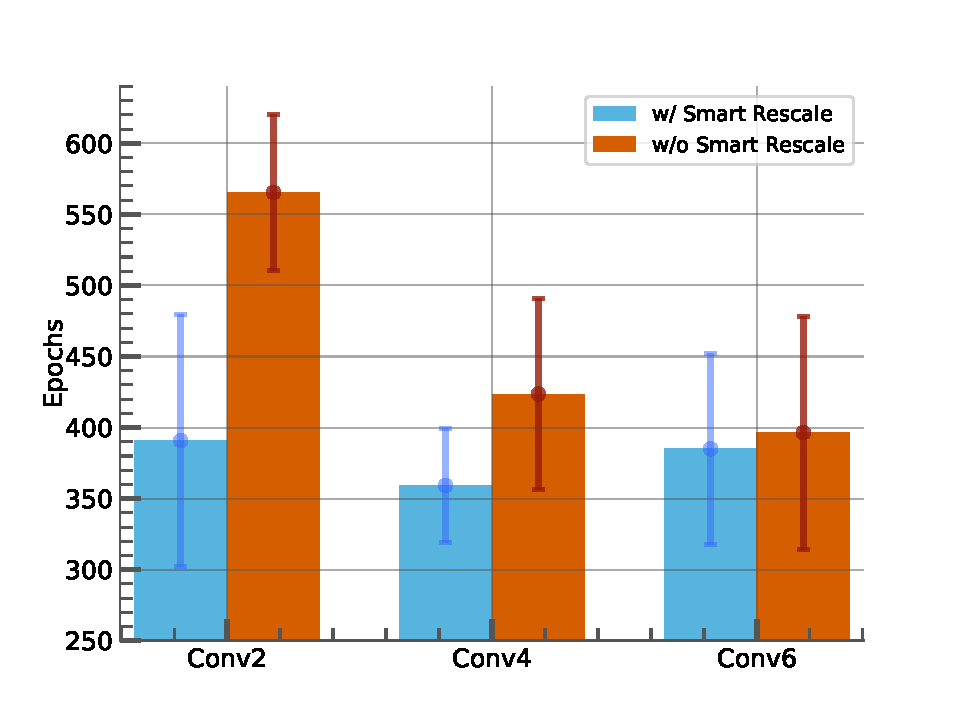
\includegraphics[width=0.49\textwidth]{chapter_2/assets/sr_impact_on_epochs_cifar10.pdf}}
  \subfloat[CIFAR-100\label{fig:chap2:rescale_cifar100}]{
    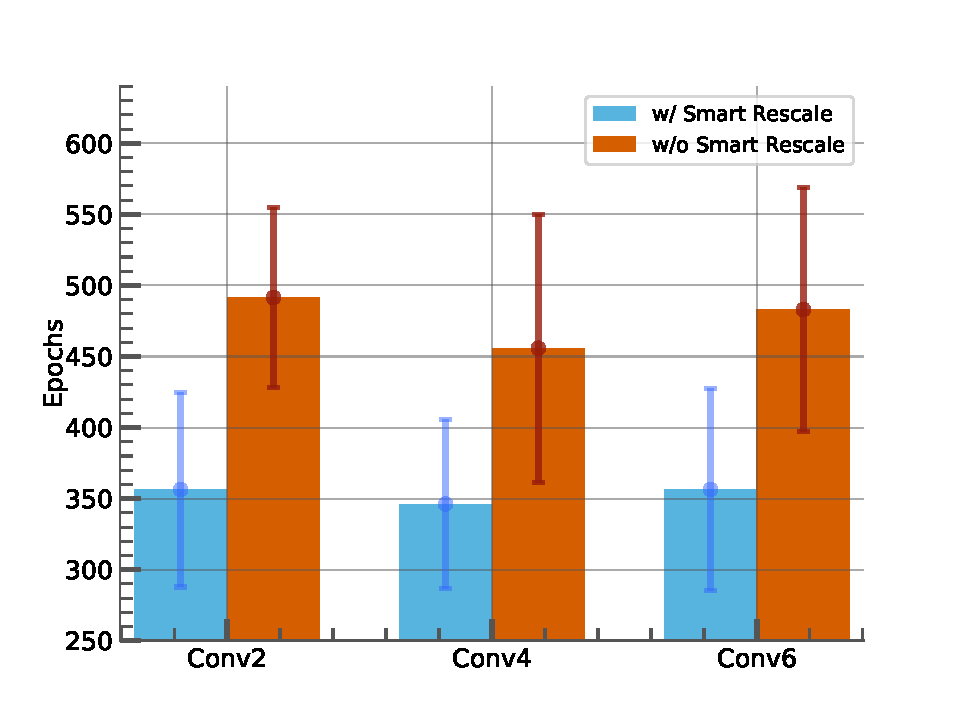
\includegraphics[width=0.49\textwidth]{chapter_2/assets/sr_impact_on_epochs_cifar100.pdf}}
  \caption{Impact of \acf{SR} on the number of epochs required to reach
    convergence for Conv\{2,4,6\} on CIFAR-10 and CIFAR-100.}
  \label{fig:chap2:rescale_impact}
\end{figure}

\subsection{Effect of the Learning Rate on Training Performances}
\label{sec:chap2:impact_learning_rate}

The learning rate is an essential hyperparameter for training neural networks as
it controls the magnitude of the network parameter updates. When training
networks with our \ac{ASLP} method introduced in this chapter, we set the
learning rate to 50. This value is significantly higher than the learning rates
typically used for training neural networks. For instance, the learning rates to
train various baseline models reported in \cite{nvidia-baselines}, are several
orders of magnitude lower than 50. An excessively high learning rate typically
results in a diverging loss function resulting in a network failing to learn a
data representation. However, in the case of \ac{ASLP}, increasing the learning
rate up to arbitrarily high values does not cause the loss function to diverge.
This section investigates the impact of the learning rate on the final
performances of the network and its convergence speed. It also provides elements
to justify the choice of a learning rate of 50.\\

\Cref{fig:chap2:lr_impact} shows the evolution of the test accuracy for Conv4,
VGG16 and ResNet-20 on CIFAR-10, when trained with different learning rates. The
solid line represents the average of five independent runs and the shaded area
of the corresponding colour indicates the standard deviation. For ease of
visualisation and comparison, the curves of test accuracies have been padded
with their last value in order to make them all 1000 epochs long. Networks have
been trained with data augmentation, \ac{WR} and \ac{SC}. Results from
\cref{fig:chap2:lr_impact} indicate that a high learning rate makes the loss
function and the accuracy converge to their final values more quickly. Networks
trained with \ac{ASLP} and a high learning rate (500 or 5000) exhibit better
performance than the ones trained with a lower learning rate (5 or 50) when
considering only the first 50 epochs. Nevertheless, the former are eventually
outperformed by the latter if the training is run for more epochs. Conversely,
an excessively low learning rate may not allow networks to reach satisfying
performance levels in a reasonable amount of time. Our experimental findings
indicate that using a scheduling policy on the learning rate does not affect
performance. In other words, opting for a high learning rate and subsequently
decreasing it yields worse results than maintaining a lower, constant learning
rate. We found that a learning rate of 50 strikes the optimal balance between
performance and training speed. Interestingly, this learning rate remains
consistent across all architectures and datasets.\\

In standard training, high learning rate values causes the optimisation to fail
because of parameters becoming too large and resulting in \ac{nan} values.
However, this is not the case for \ac{ASLP} which exhibit robustness to high
learning rates. This robustness can be attributed to the fact that, in
\ac{ASLP}, the trained variables are the latent masks, denoted by
$\bm{\hat{m}}$, which can be interpreted as probabilities of selection by
applying a sigmoid function (refer to
\cref{sec:chap2:stochastic-sampling,prop:chap2:probability-interpretation}). The
sigmoid function ensures that: \emph{(i)} the latent masks cannot take extreme
values leading to \ac{nan} because of increasingly small gradients as the latent
masks move away from the origin (see \cref{sec:chap2:stochastic-sampling}), and
\emph{(ii)} the sigmoid output is bounded between 0 and 1 resulting in
probabilities of selection close to 0 or 1, but not altering in a dramatical way
the output of the network that otherwise might also lead to \ac{nan} values.
Besides, due to the vanishingly small gradients as the masks move further away
from the origin, it is practically impossible to reactivate those weights, let
alone reactivate them with a smaller learning rate. This accounts for the
observation that reducing the learning rate after using a high learning rate
does not enhance performance.\\

\begin{figure}[htbp]
  \centering
  \subfloat[Conv4\label{fig:chap2:lr_conv4}]{
    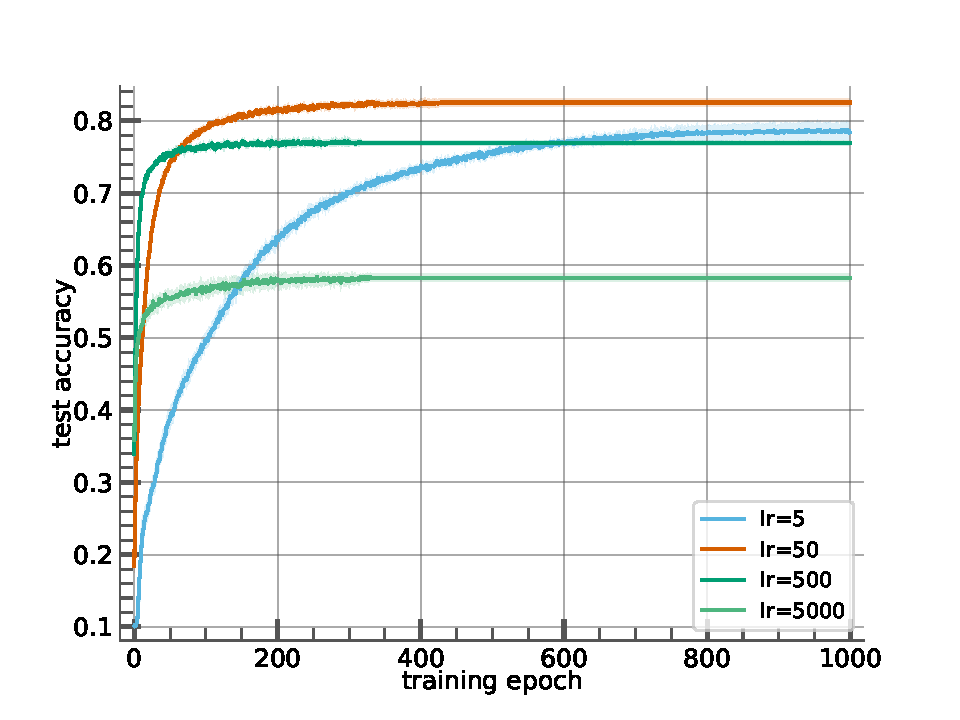
\includegraphics[width=0.33\linewidth]{chapter_2/assets/impact_of_lr_Conv4.pdf}}
  \subfloat[VGG16\label{fig:chap2:lr_vgg16}]{
    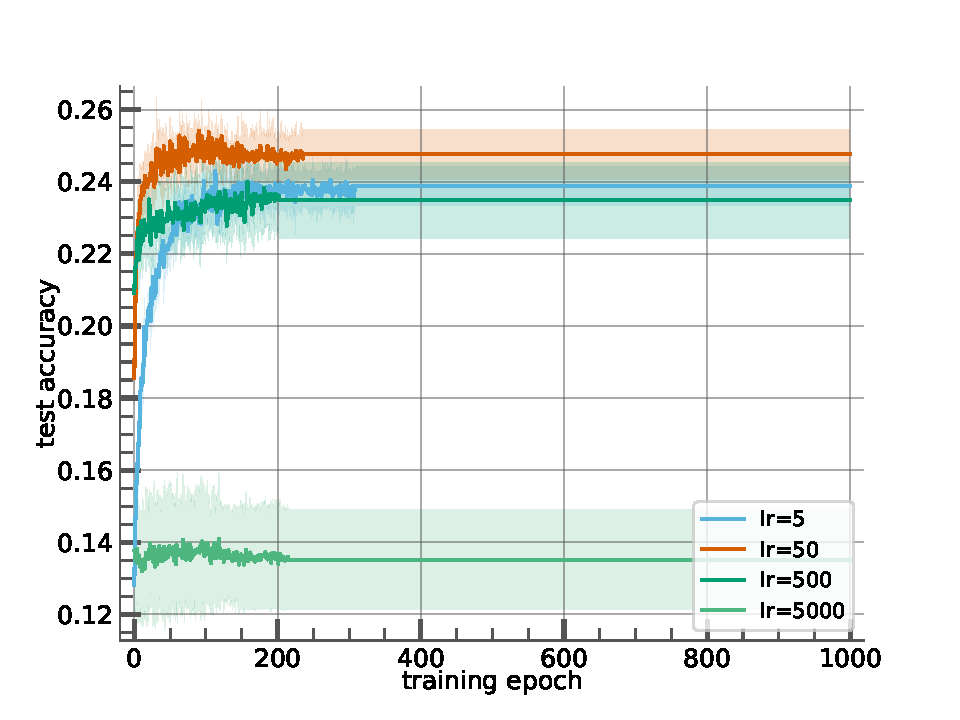
\includegraphics[width=0.33\linewidth]{chapter_2/assets/impact_of_lr_PrunableVGG16.pdf}}
  \subfloat[ResNet-20\label{fig:chap2:lr_resnet20}]{
    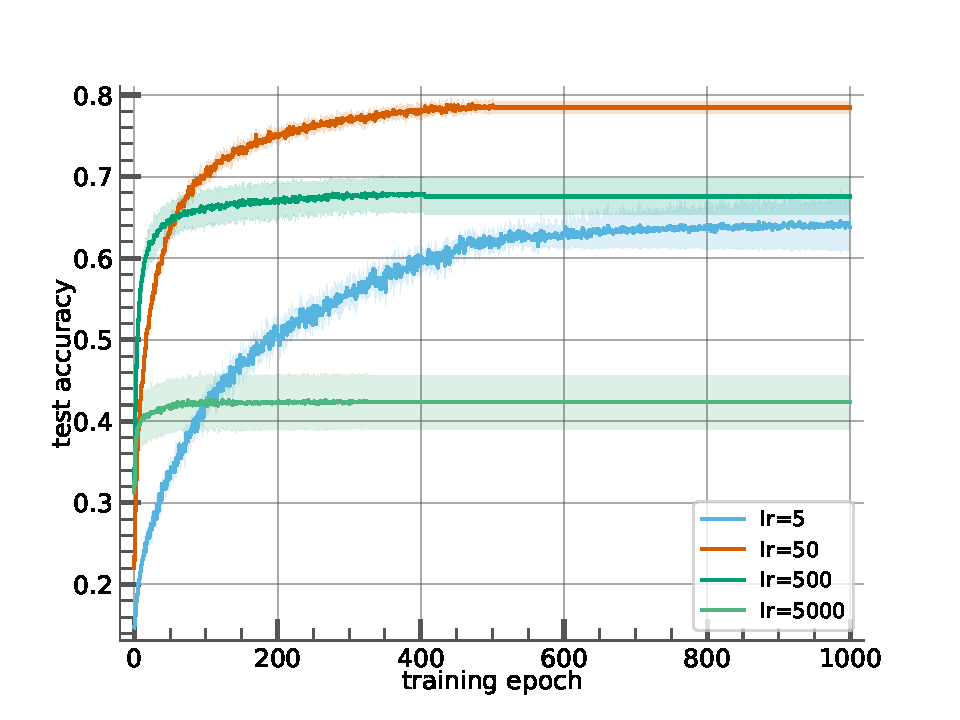
\includegraphics[width=0.33\linewidth]{chapter_2/assets/impact_of_lr_PrunableResNet20.pdf}}
  \caption{Evolution of the test accuracy for Conv4, VGG16 and ResNet-20 trained
    with \ac{ASLP} (with data augmentation, \ac{WR} and \ac{SC}) on CIFAR-10 for various learning
    rates. A learning rate of 50 yields the optimal balance between performance
    and training speed.}
  \label{fig:chap2:lr_impact}
\end{figure}

\subsection{Post Training Pruning Rate Adjustment}
\label{sec:chap2:increasing_sparsity}

This section investigates the impact of pruning a network trained with \ac{ASLP}
to a given pruning rate instead of using the \emph{thresholding} strategy,
described in \cref{sec:chap2:freezing_topology}. Unlike Edge-popup
\cite{DBLP:conf/cvpr/RamanujanWKFR20} where the pruning rate is a hyperparameter
of the method, the proposed \ac{ASLP} approach does not enforce a predefined
pruning rate during training. Instead, it determines an optimal subset of
weights that enables the network to minimises the loss function by updating
weights probabilities of selection $p_{ij}$ through backpropagation
\cite{rumelhart1986learning}. Rather than being enforced, the pruning rate is
observed and is determined by thresholding the $p_{ij}$ following
\cref{eq:chap2:pruning}, as explained in \cref{sec:chap2:freezing_topology}. The
observed pruning rate, which is the fraction of weights whose probabilities of
selection $p_{ij}$ are smaller than the threshold $\tau$ in
\cref{eq:chap2:pruning}, lies just above 50\% for the tested architectures (60\%
for VGG16), as reported in \cref{tab:chap2:observed_sparsity}. However, instead
of thresholding the $p_{ij}$ and observing the pruning rate, it can be adjusted
by pruning the weights on the magnitude of their associated latent masks
$\bm{\hat{m}}$, which enforces the pruning rate \emph{a posteriori} by
considering the probabilities of selection $p_{ij}$ as saliency scores. This is
equivalent to changing the value of the threshold $\tau$ in
\cref{eq:chap2:pruning} in order to match a given pruning rate. Notably,
Conv\{2,4,6\} networks trained with \ac{ASLP}, and pruned a posteriori with a
given pruning rate, achieve compelling performances on CIFAR-10 and CIFAR-100
datasets for pruning rates up to 85\%, whereas their observed pruning rate is
approximately 50\% (see
\cref{fig:chap2:sparsity_impact,tab:chap2:observed_sparsity}). In the
\cref{fig:chap2:sparsity_impact}, the solid line represents the average test
accuracy of five independent runs and the shaded area represents the standard
deviation.\\

Moreover, the results presented in \cref{fig:chap2:sparsity_impact} provide
further support for the \textit{thresholding} strategy. This figure displays the
test accuracy of networks trained with \ac{ASLP} and pruned a posteriori, as
described in the above paragraph, for various pruning rates. Sweeping through
the pruning rate enables us to determine the optimal pruning rate for each
network and dataset combination. The optimal pruning rate is defined as the
pruning rate that yields the highest test accuracy. The results presented in the
figure suggest that the optimal pruning rate for Conv\{2,4,6\} and ResNet-20
networks lies at 50\%, and at 60\% for VGG16. These rates are precisely the
observed pruning rates obtained using the \ac{ASLP} method with the
\emph{thresholding} pruning strategy (see \cref{tab:chap2:observed_sparsity}).
In other words, the \ac{ASLP} method together with \emph{thresholding} pruning
automatically determine the optimal pruning rate for an architecture without the
need for a costly grid search, in contrary to the Edge-popup method
\cite{DBLP:conf/cvpr/RamanujanWKFR20}.\\

\begin{figure}[htbp]
  \centering
  \subfloat[cifar10\label{fig:chap2:sparsity_cifar10}]{
    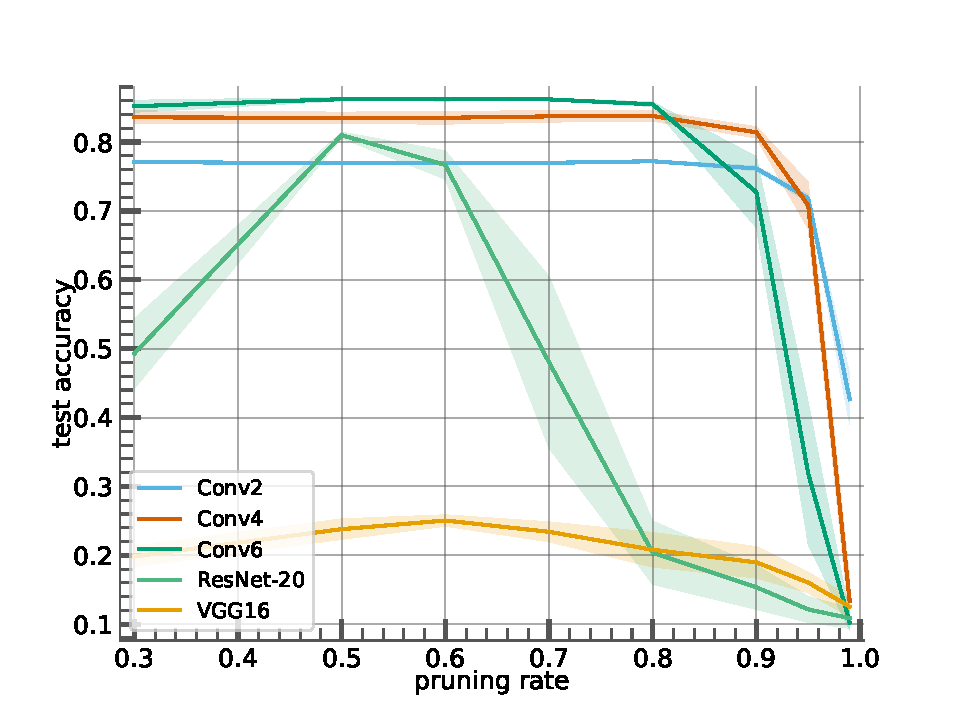
\includegraphics[width=0.49\textwidth]{chapter_2/assets/impact_of_pr_cifar10.pdf}}
    \subfloat[cifar100\label{fig:chap2:sparsity_cifar100}]{
    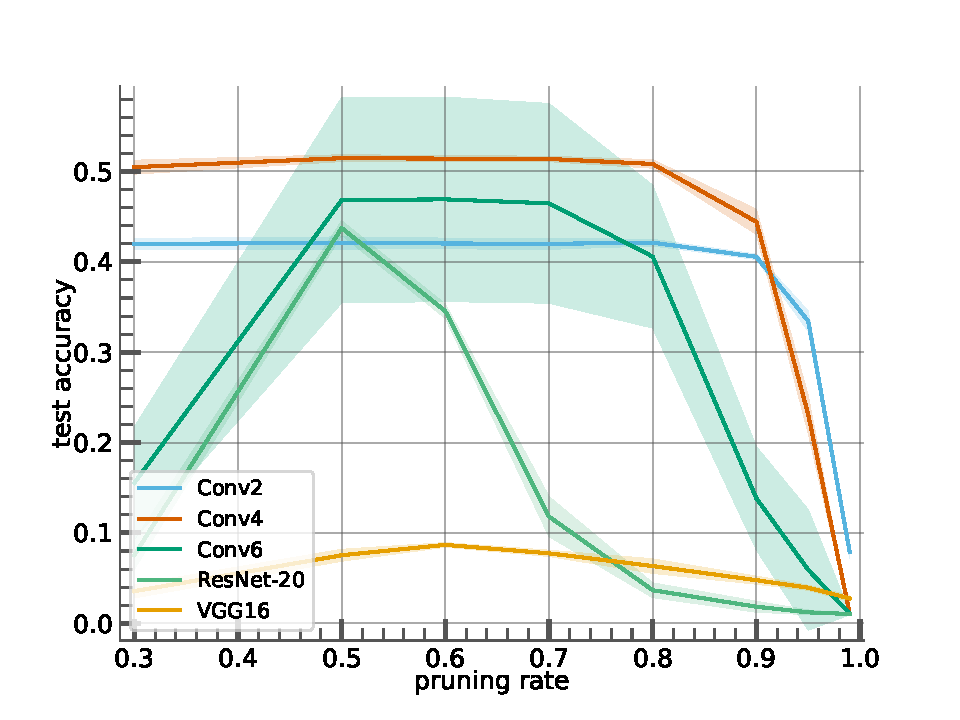
\includegraphics[width=0.49\textwidth]{chapter_2/assets/impact_of_pr_cifar100.pdf}}
    \caption{Comparative analysis of \ac{ASLP} performance for CIFAR-10 and CIFAR-100
    datasets using various network architectures (Conv\{2,4,6\}, ResNet-20, and
    VGG16) at different pruning rates. \ac{ASLP} performances are evaluated with
    \ac{WR}, \ac{SC} and data augmentation. Results demonstrate that
    Conv\{2,4,6\} networks maintain strong performance even at higher pruning
    rates and indicate that the pruning rate achieved by thresholding is
    equivalent to the pruning rate yielding the best test accuracy when sweeping
    through the possible pruning rates.}
  \label{fig:chap2:sparsity_impact}
\end{figure}


\section{Conclusion}\label{sec:chap2:conclusion}
% region : Conclusion

In this chapter, we introduced the \acl{ASLP} method, which focuses on selecting
efficient subnetworks from large, untrained neural networks through stochastic
pruning, without training the weights. \acl{ASLP} is a stochastic subnetwork
selection method that uses \acl{GS} sampling and a new mask parametrisation to
optimize the subnetwork topology while mitigating numerical instabilities.
Additionally, we presented the \acl{SR} technique to accelerate training and
improve the accuracy of the resulting subnetworks. Our experimental results show
that \ac{ASLP} outperforms state-of-the-art methods, such as Edge-popup
\cite{DBLP:conf/cvpr/RamanujanWKFR20} and Supermask
\cite{DBLP:conf/nips/ZhouLLY19}, on the CIFAR-10 and CIFAR-100 datasets across
various network architectures. Our proposed \textit{thresholding} pruning
strategy consistently yields better performance than Supermask
\textit{averaging} approach, while finding the optimal pruning rate without the
need for costly grid-search, in contrary to Edge-popup. Furthermore, our
\acl{SR} method leads to faster convergence and improved accuracy with a lower
overhead compared to other weight-rescaling techniques, such as \acl{DWR}.
\acl{ASLP} also exhibits robustness to substantially high learning rates,
ensuring stable performance across different network architectures and
datasets.\\

All in all, the \acl{ASLP} method provides a promising solution for selecting
efficient subnetworks from large untrained neural networks through stochastic
pruning, offering improved performance and faster convergence and a new
perspective on neural network training which focuses on topology selection
rather than weight training.

% TODO: ajouter la partie qui lie le prochain chapitre.

% \textit{Ajouter la partie qui lie le prochain chapitre.}

%endregion : conclusion
